% =====================================================================
%  RAPPORT DE PROJET DE FIN DE MODULE
%  Systeme Intelligent de Controle Qualite des Impellers
%  Filiere BDIA1 - Annee universitaire 2025-2026
% =====================================================================
\documentclass[12pt,a4paper,openany]{report}

% ---------- Encoding & langue ----------
\usepackage[utf8]{inputenc}
\usepackage[T1]{fontenc}
\usepackage[french]{babel}
\usepackage{lmodern}
\usepackage{microtype}

% ---------- Mise en page ----------
\usepackage[a4paper,margin=2.5cm,headheight=15pt]{geometry}
\usepackage{setspace}
\onehalfspacing
\usepackage{parskip}
\usepackage{fancyhdr}
\usepackage{titlesec}
\usepackage{enumitem}
\setlist{itemsep=2pt,topsep=4pt}
\usepackage{epigraph}

% ---------- Graphiques & tableaux ----------
\usepackage{graphicx}
\usepackage{float}
\usepackage{caption}
\usepackage{subcaption}
\captionsetup{font=small,labelfont=bf}
\graphicspath{{images/}}
\usepackage{array}
\usepackage{booktabs}
\usepackage{longtable}
\usepackage{tabularx}
\usepackage{multirow}
\usepackage{makecell}

% ---------- Couleurs ----------
\usepackage[dvipsnames]{xcolor}
\definecolor{primary}{RGB}{0,90,160}
\definecolor{accent}{RGB}{200,80,30}
\definecolor{softgray}{RGB}{240,240,245}
\definecolor{codebg}{RGB}{248,248,248}
\definecolor{codekw}{RGB}{0,90,160}
\definecolor{codestr}{RGB}{170,55,30}
\definecolor{codecmt}{RGB}{100,110,100}

% ---------- Boites ----------
\usepackage[most]{tcolorbox}
\newtcolorbox{infobox}[1][]{enhanced,colback=softgray,colframe=primary,
  fonttitle=\bfseries,coltitle=white,colbacktitle=primary,
  boxrule=0.4pt,arc=2pt,left=8pt,right=8pt,top=4pt,bottom=4pt,#1}
\newtcolorbox{warnbox}[1][]{enhanced,colback=accent!8,colframe=accent,
  fonttitle=\bfseries,coltitle=white,colbacktitle=accent,
  boxrule=0.4pt,arc=2pt,left=8pt,right=8pt,top=4pt,bottom=4pt,#1}

% ---------- Code ----------
\usepackage{listings}
\lstdefinestyle{pystyle}{
  language=Python,
  backgroundcolor=\color{codebg},
  basicstyle=\ttfamily\footnotesize,
  keywordstyle=\color{codekw}\bfseries,
  stringstyle=\color{codestr},
  commentstyle=\color{codecmt}\itshape,
  numbers=left, numberstyle=\tiny\color{gray}, numbersep=6pt,
  frame=single, rulecolor=\color{gray!40},
  breaklines=true, breakatwhitespace=true,
  showstringspaces=false,
  tabsize=2, captionpos=b,
  literate=
    {e}{{\'e}}1 {e}{{\`e}}1 {e}{{\^e}}1 {a}{{\`a}}1 {a}{{\^a}}1
    {i}{{\^\i}}1 {o}{{\^o}}1 {u}{{\`u}}1 {u}{{\^u}}1 {c}{{\c c}}1
}
\lstset{style=pystyle}

% ---------- Mathematiques ----------
\usepackage{amsmath,amssymb,amsfonts}

% ---------- Acronymes ----------
\usepackage[acronym,nonumberlist,toc]{glossaries}
\makeglossaries

\newacronym{ia}{IA}{Intelligence Artificielle}
\newacronym{dl}{DL}{Deep Learning (apprentissage profond)}
\newacronym{ml}{ML}{Machine Learning (apprentissage automatique)}
\newacronym{cnn}{CNN}{Convolutional Neural Network}
\newacronym{mlp}{MLP}{Multi-Layer Perceptron}
\newacronym{tl}{TL}{Transfer Learning (apprentissage par transfert)}
\newacronym{cv}{CV}{Computer Vision}
\newacronym{qc}{QC}{Quality Control (controle qualite)}
\newacronym{cao}{CAO}{Conception Assistee par Ordinateur}
\newacronym{relu}{ReLU}{Rectified Linear Unit}
\newacronym{bn}{BN}{Batch Normalization}
\newacronym{sgd}{SGD}{Stochastic Gradient Descent}
\newacronym{lr}{LR}{Learning Rate (taux d'apprentissage)}
\newacronym{auc}{AUC}{Area Under the Curve}
\newacronym{roc}{ROC}{Receiver Operating Characteristic}
\newacronym{tpr}{TPR}{True Positive Rate}
\newacronym{fpr}{FPR}{False Positive Rate}
\newacronym{fn}{FN}{Faux Negatif}
\newacronym{fp}{FP}{Faux Positif}
\newacronym{ap}{AP}{Average Precision}
\newacronym{api}{API}{Application Programming Interface}
\newacronym{gpu}{GPU}{Graphics Processing Unit}
\newacronym{cpu}{CPU}{Central Processing Unit}
\newacronym{rgb}{RGB}{Red Green Blue}
\newacronym{tf}{TF}{TensorFlow}
\newacronym{tflite}{TFLite}{TensorFlow Lite}

% ---------- Hyperliens ----------
\usepackage[hidelinks,colorlinks=true,linkcolor=primary,urlcolor=primary,citecolor=accent]{hyperref}

% ---------- Style des chapitres / sections ----------
\titleformat{\chapter}[hang]{\Huge\bfseries\color{primary}}{\thechapter.}{1em}{}
\titlespacing*{\chapter}{0pt}{-20pt}{20pt}
\titleformat{\section}{\Large\bfseries\color{primary}}{\thesection}{0.6em}{}
\titleformat{\subsection}{\large\bfseries\color{accent}}{\thesubsection}{0.5em}{}

% ---------- En-tete / pied de page ----------
\pagestyle{fancy}
\fancyhf{}
\renewcommand{\headrulewidth}{0.4pt}
\renewcommand{\footrulewidth}{0pt}
\fancyhead[L]{\small\textit{Controle Qualite Intelligent des Impellers}}
\fancyhead[R]{\small\textit{BDIA1 - 2025/2026}}
\fancyfoot[C]{\thepage}

% =====================================================================
\begin{document}

% =====================================================================
%  PAGE DE GARDE
% =====================================================================
\begin{titlepage}
\centering
\vspace*{0.3cm}

{\Large\textbf{Universite / Ecole d'Ingenieurs} \par}
{\large Filiere BDIA1 --- Big Data \& Intelligence Artificielle \par}
\vspace{0.4cm}

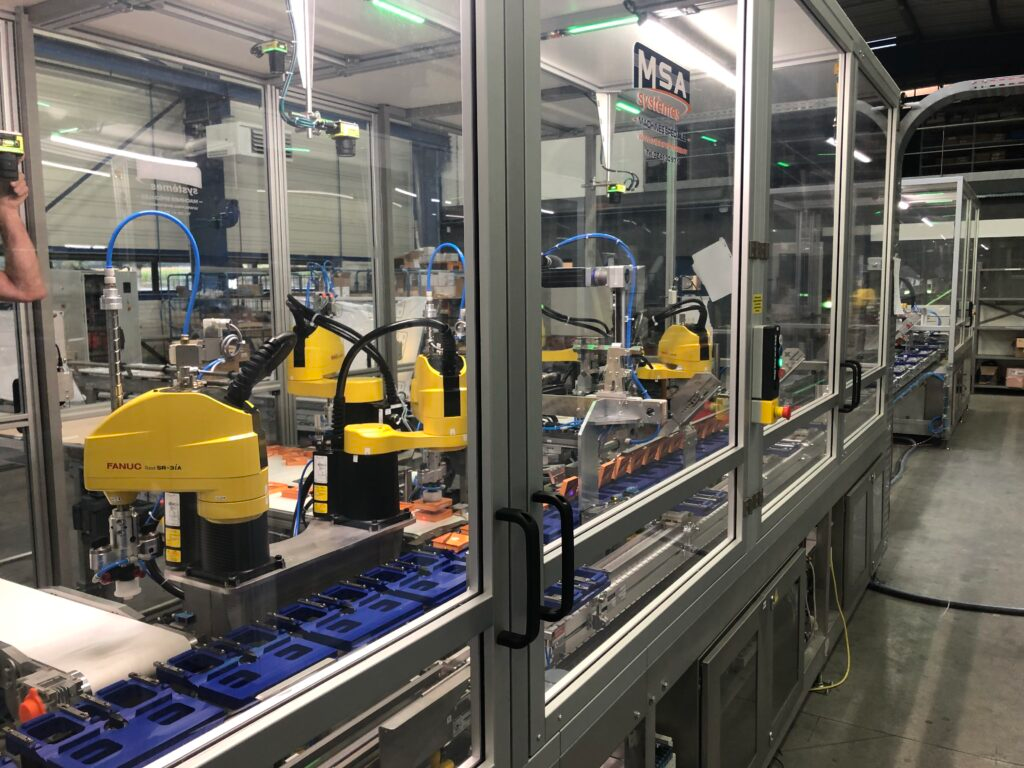
\includegraphics[width=0.32\textwidth]{image1.png}\\[0.6cm]

\rule{\textwidth}{1.4pt}\\[0.4cm]
{\Huge\bfseries\color{primary} Systeme Intelligent\\[0.2cm] de Controle Qualite\\[0.2cm] des Impellers \par}
\vspace{0.3cm}
\rule{\textwidth}{1.4pt}\\[0.6cm]

{\large\itshape Detection automatique des defauts de fonderie\\
par Apprentissage Profond et Transfer Learning \par}

\vspace{1.2cm}

{\large\bfseries Rapport de projet de fin de module\\
\textit{Module : Apprentissage Profond et Vision par Ordinateur}}

\vspace{1.2cm}

\begin{minipage}[t]{0.46\textwidth}
\raggedright
{\large\bfseries Realise par~:}\\[0.3cm]
{\large
Ayoub \textsc{El-Moujahid}\\
Mohamed \textsc{Errahmouni}\\
Soulama Doubie Judicael Noe\\
Hazem \textsc{Douzi}
}
\end{minipage}\hfill
\begin{minipage}[t]{0.46\textwidth}
\raggedleft
{\large\bfseries Encadre par~:}\\[0.3cm]
{\large Prof. Dr Naoual \textsc{Attaoui}}
\end{minipage}

\vfill

{\large Annee universitaire \textbf{2025--2026}}\\[0.4cm]
\vspace{0.2cm}
\end{titlepage}

% =====================================================================
%  REMERCIEMENTS
% =====================================================================
\chapter*{Remerciements}
\addcontentsline{toc}{chapter}{Remerciements}
\thispagestyle{fancy}

Au terme de ce projet de fin de module, nous tenons a exprimer notre profonde gratitude a toutes les personnes qui, par leur soutien, leurs conseils et leur disponibilite, ont contribue de pres ou de loin a son aboutissement.

Nos remerciements les plus sinceres s'adressent en premier lieu a notre encadrante, \textbf{Madame le Professeur Dr Naoual Attaoui}, pour la qualite de son encadrement, la rigueur scientifique de ses orientations et la confiance qu'elle nous a accordee tout au long de ce travail. Sa pedagogie et ses remarques eclairees ont constitue un guide precieux durant chaque etape de la realisation.

Nous remercions egalement l'ensemble du corps professoral de la filiere \textbf{BDIA1 (Big Data \& Intelligence Artificielle)} pour la qualite des enseignements dispenses, qui ont jete les fondations theoriques et pratiques sur lesquelles repose ce projet.

Notre reconnaissance va aussi a la communaute open-source --- en particulier aux equipes de \textsc{TensorFlow}, \textsc{Keras}, \textsc{PyTorch}, \textsc{Scikit-learn} et \textsc{Matplotlib} --- ainsi qu'a Ravirajsinh Dabhi qui a publie sur Kaggle le jeu de donnees \emph{Casting Defect Detection} sans lequel ce travail n'aurait pas ete possible.

Enfin, nous adressons un remerciement chaleureux a nos familles et a nos camarades de promotion pour leur soutien moral indefectible et l'enrichissement intellectuel mutuel qui a caracterise notre annee universitaire.

\vspace{1.5cm}
\hfill\textit{Les auteurs}

% =====================================================================
%  RESUME (FR) + ABSTRACT (EN)
% =====================================================================
\chapter*{Resume}
\addcontentsline{toc}{chapter}{Resume}
\thispagestyle{fancy}

Dans le secteur de la fonderie, le controle qualite des pieces metalliques --- en particulier des \emph{impellers} (roues de pompes centrifuges) --- represente un enjeu industriel majeur. Realise traditionnellement de maniere visuelle par des operateurs humains, ce controle souffre d'une triple limite~: il est lent, subjectif et sujet a la fatigue. Une seule piece defectueuse non detectee peut provoquer une defaillance en service avec des consequences couteuses pour le client final.

Le present rapport propose un \textbf{systeme intelligent de controle qualite automatique} fonde sur la \emph{vision par ordinateur} et l'\emph{apprentissage profond}. Trois familles de modeles sont developpees, comparees et discutees suivant une demarche progressive~: (i) un \textbf{Perceptron Multi-Couches (MLP)} servant de \emph{baseline}, (ii) un \textbf{Reseau de Neurones Convolutif (CNN)} entraine de zero, et (iii) un modele de \textbf{Transfer Learning} fonde sur l'architecture \textsc{EfficientNetB0} pre-entrainee sur \textsc{ImageNet}.

Une attention particuliere est portee a la chaine de pretraitement, developpee en double implementation \textsc{TensorFlow} (\texttt{tf.data}) et \textsc{PyTorch} (\texttt{DataLoader}) afin de garantir reproductibilite, modularite et portabilite. Cette chaine integre la normalisation \emph{ImageNet}, des transformations \emph{color balancing} (white balance, equalisation d'histogramme, channel shuffle), des augmentations geometriques et photometriques, ainsi qu'une gestion explicite du desequilibre des classes par \emph{class weights} ou \texttt{WeightedRandomSampler}.

Le modele final atteint une \textbf{accuracy de 99{,}44\%} et un \textbf{AUC de 0{,}9993} sur l'ensemble de test, avec un \emph{recall} de \textbf{99{,}34\%} sur la classe defectueuse --- metrique critique en controle qualite industriel. Ces performances, obtenues avec seulement 6\,600 images d'entrainement, demontrent la pertinence du \emph{Transfer Learning} pour les problemes de classification industrielle a faible volume de donnees.

\vspace{0.4cm}
\noindent\textbf{Mots-cles~:} Controle qualite, Fonderie, Impeller, Apprentissage profond, Reseaux de neurones convolutifs, Transfer Learning, EfficientNet, TensorFlow, PyTorch, Vision par ordinateur, Detection de defauts.

\chapter*{Abstract}
\addcontentsline{toc}{chapter}{Abstract}
\thispagestyle{fancy}

In the foundry industry, quality control of metallic parts --- particularly \emph{impellers} (centrifugal pump wheels) --- represents a major industrial challenge. Traditionally performed visually by human operators, such inspection suffers from three intrinsic limitations~: it is slow, subjective, and prone to fatigue-induced errors. A single undetected defective part can lead to in-service failure with costly consequences for the end customer.

This report proposes an \textbf{intelligent automatic quality control system} based on \emph{computer vision} and \emph{deep learning}. Three model families are developed, compared, and discussed following a progressive approach~: (i) a \textbf{Multi-Layer Perceptron (MLP)} as a baseline, (ii) a \textbf{Convolutional Neural Network (CNN)} trained from scratch, and (iii) a \textbf{Transfer Learning} model based on the \textsc{EfficientNetB0} architecture pre-trained on \textsc{ImageNet}.

Special attention is devoted to the preprocessing pipeline, developed in dual implementation \textsc{TensorFlow} (\texttt{tf.data}) and \textsc{PyTorch} (\texttt{DataLoader}) to ensure reproducibility, modularity and portability. The pipeline integrates \emph{ImageNet} normalization, \emph{color balancing} transformations (white balance, histogram equalization, channel shuffle), geometric and photometric augmentations, as well as explicit class imbalance handling through \emph{class weights} or \texttt{WeightedRandomSampler}.

The final model achieves \textbf{99.44\% accuracy} and an \textbf{AUC of 0.9993} on the test set, with \textbf{99.34\% recall} on the defective class --- the critical metric in industrial quality control. These results, obtained with only 6{,}600 training images, demonstrate the relevance of \emph{Transfer Learning} for industrial classification problems with limited data.

\vspace{0.4cm}
\noindent\textbf{Keywords:} Quality Control, Foundry, Impeller, Deep Learning, Convolutional Neural Networks, Transfer Learning, EfficientNet, TensorFlow, PyTorch, Computer Vision, Defect Detection.

% =====================================================================
%  SOMMAIRES
% =====================================================================
\tableofcontents
\thispagestyle{fancy}

\listoffigures
\addcontentsline{toc}{chapter}{Liste des figures}
\thispagestyle{fancy}

\listoftables
\addcontentsline{toc}{chapter}{Liste des tableaux}
\thispagestyle{fancy}

\printglossary[type=\acronymtype,title={Liste des acronymes},toctitle={Liste des acronymes}]

% =====================================================================
%  INTRODUCTION GENERALE
% =====================================================================
\chapter{Introduction generale}

\section{Contexte general}

La quatrieme revolution industrielle, communement designee sous le terme \emph{Industrie 4.0}, redefinit en profondeur les processus de production manufacturiere. Au c\oe ur de cette transformation se trouve l'integration massive de technologies numeriques --- objets connectes, jumeaux numeriques, robotique collaborative et, plus particulierement, \emph{intelligence artificielle} --- au sein des chaines de fabrication. Dans ce contexte, le \textbf{controle qualite automatique} apparait comme l'une des applications a plus forte valeur ajoutee~: il conditionne directement la fiabilite des produits livres, la satisfaction client et la rentabilite des installations.

La fonderie, secteur historique et strategique de l'industrie metallurgique, n'echappe pas a cette mutation. Les pieces issues du moulage --- particulierement les composants critiques tels que les \emph{impellers} de pompes centrifuges --- doivent satisfaire a des specifications dimensionnelles et de surface tres exigeantes. Tout ecart (fissure, deformation, bavure, porosite) peut compromettre la fonction hydraulique de la pompe et entrainer une defaillance prematuree, parfois catastrophique, en service.

\section{Problematique}

Le controle qualite des impellers en sortie de chaine de fonderie est aujourd'hui realise selon deux approches~:

\begin{itemize}
    \item \textbf{Inspection visuelle manuelle.} Un operateur examine chaque piece a l'\oe il nu et la classe comme conforme ou defectueuse. Cette methode est universelle mais souffre de trois limites majeures~: \emph{lenteur} (cadence de production limitee), \emph{subjectivite} (variabilite inter-operateurs et intra-operateur), et \emph{fatigue} (taux d'erreur croissant en fin de poste).
    \item \textbf{Controle non destructif (CND) instrumente.} Radiographie, ressuage, ultrasons. Tres precis mais couteux, lents et inadaptes a un controle de masse a 100\,\%.
\end{itemize}

Aucune de ces deux approches ne permet a la fois un controle \emph{exhaustif}, \emph{rapide} et \emph{reproductible} en ligne. Cette limitation conduit, dans la pratique industrielle, a l'application d'un controle par echantillonnage statistique --- ce qui laisse mecaniquement passer une fraction de pieces defectueuses chez le client.

\begin{infobox}[title=Question de recherche]
Est-il possible de concevoir un systeme automatique, capable de classifier en quelques millisecondes une image de piece comme \texttt{conforme} ou \texttt{defectueuse}, avec une precision suffisante pour un deploiement industriel et un \emph{recall} eleve sur la classe defectueuse afin de minimiser les faux negatifs~?
\end{infobox}

\section{Objectifs du projet}

Pour repondre a cette problematique, le present projet poursuit les objectifs suivants~:

\begin{enumerate}
    \item \textbf{Etudier} les principes et l'etat de l'art de la classification d'images par apprentissage profond, en particulier les architectures convolutives et le \emph{Transfer Learning}.
    \item \textbf{Concevoir} une chaine de pretraitement reproductible et portable, adaptee aux contraintes des images industrielles (variations d'eclairage, angles, textures de surface).
    \item \textbf{Implementer et comparer} trois modeles de classification representatifs d'une progression methodologique~: \gls{mlp}, \gls{cnn} et Transfer Learning sur \textsc{EfficientNetB0}.
    \item \textbf{Evaluer rigoureusement} les performances obtenues a l'aide de metriques industriellement pertinentes (\emph{accuracy}, \emph{precision}, \emph{recall}, F1-score, \gls{auc}) et d'une analyse fine des erreurs (faux negatifs, faux positifs).
    \item \textbf{Discuter} les limites du systeme propose et formuler des perspectives pour son industrialisation effective (deploiement embarque, multi-classes, localisation).
\end{enumerate}

\section{Methodologie generale}

La demarche methodologique adoptee s'inscrit dans une logique \emph{incrementale} et \emph{comparative}~:

\begin{enumerate}
    \item \textbf{Acquisition} d'un jeu de donnees public reconnu (\emph{Casting Defect Detection}, Kaggle).
    \item \textbf{Exploration et pretraitement} avec une double implementation TensorFlow / PyTorch pour valider la robustesse du pipeline.
    \item \textbf{Modelisation progressive}~: chaque modele est entraine, evalue, ses limites identifiees, et la generation suivante est concue pour les depasser.
    \item \textbf{Evaluation finale} sur un ensemble de test \emph{strictement disjoint}, jamais vu durant l'apprentissage.
    \item \textbf{Analyse critique} des resultats et des erreurs residuelles dans une perspective de deploiement industriel.
\end{enumerate}

\section{Organisation du rapport}

Ce rapport est structure en \textbf{huit chapitres}~:
\begin{description}[leftmargin=2.2cm,style=nextline]
    \item[Chapitre~1] La presente introduction generale.
    \item[Chapitre~2] Etat de l'art du controle qualite par vision artificielle et apprentissage profond.
    \item[Chapitre~3] Procede de fonderie en moule carapace et typologie des defauts observes sur les impellers.
    \item[Chapitre~4] Acquisition, organisation et exploration du jeu de donnees.
    \item[Chapitre~5] Conception detaillee du pipeline de pretraitement (TensorFlow et PyTorch).
    \item[Chapitre~6] Modelisation~: \gls{mlp}, \gls{cnn} et Transfer Learning avec \textsc{EfficientNetB0}.
    \item[Chapitre~7] Evaluation finale, analyse des erreurs et discussion industrielle.
    \item[Chapitre~8] Conclusion generale et perspectives.
\end{description}

% =====================================================================
%  ETAT DE L'ART
% =====================================================================
\chapter{Etat de l'art}

\section{Controle qualite industriel par vision artificielle}

Le controle qualite par vision artificielle (\emph{Machine Vision}) est une discipline ancienne, dont les premiers systemes industriels remontent aux annees 1980. Historiquement, ces systemes reposaient sur des \emph{regles expertes} fondees sur le traitement d'image classique~: seuillage adaptatif, detection de contours (filtres de Sobel, Canny), morphologie mathematique, et descripteurs de texture (matrices de co-occurrence, ondelettes de Gabor). Ces approches, performantes sur des defauts simples et bien definis, montrent rapidement leurs limites des que l'on s'attaque a des defauts \emph{visuellement variables} --- tels que les fissures fines, les deformations subtiles ou les bavures heterogenes que l'on rencontre en fonderie.

L'avenement de l'apprentissage profond, et plus precisement des reseaux convolutifs \cite{lecun1998}, a profondement bouleverse ce paysage. La capacite des CNN a apprendre automatiquement des representations hierarchiques des images --- des contours de bas niveau aux concepts semantiques de haut niveau --- a permis des progres considerables, comme illustre par la victoire d'\textsc{AlexNet} \cite{krizhevsky2012} a la competition \textsc{ILSVRC} 2012 sur \textsc{ImageNet}. Depuis, le \emph{deep learning} s'est impose comme l'approche dominante pour la classification d'images, et son adoption dans le controle qualite industriel s'est rapidement generalisee.

\section{Architectures convolutives marquantes}

\subsection{Les jalons historiques}

\begin{itemize}
    \item \textbf{LeNet-5} \cite{lecun1998}~: premier CNN moderne, applique a la reconnaissance de chiffres manuscrits. Pose les bases (convolution, pooling, couches denses).
    \item \textbf{AlexNet} \cite{krizhevsky2012}~: 8 couches, exploitation du GPU, fonctions d'activation \gls{relu}, \emph{dropout}. Marque le debut de l'ere \emph{deep}.
    \item \textbf{VGGNet} \cite{simonyan2014}~: empilement profond (16 a 19 couches) de petits filtres $3\times 3$. Demonstration que la profondeur ameliore la performance.
    \item \textbf{ResNet} \cite{he2016}~: introduction des connexions residuelles (\emph{skip connections}), permettant d'entrainer des reseaux jusqu'a 152 couches sans degradation.
    \item \textbf{Inception / GoogLeNet} \cite{szegedy2015}~: \emph{Inception modules} parallelisant plusieurs tailles de filtres dans un meme bloc.
\end{itemize}

\subsection{EfficientNet : etat de l'art recent}

\textsc{EfficientNet} \cite{tan2019efficientnet}, introduit par Tan et Le en 2019, propose une approche systematique de \emph{compound scaling}~: au lieu de faire croitre arbitrairement la profondeur, la largeur ou la resolution d'entree, les auteurs montrent qu'il est optimal de \emph{conjointement} augmenter ces trois dimensions selon un facteur unique~$\phi$~:
\begin{equation}
    \text{depth: } d = \alpha^\phi, \quad
    \text{width: } w = \beta^\phi, \quad
    \text{resolution: } r = \gamma^\phi
\end{equation}
sous la contrainte $\alpha\cdot\beta^2\cdot\gamma^2 \approx 2$. Le bloc fondamental d'EfficientNet est le \emph{Mobile Inverted Bottleneck} (\textsc{MBConv}), enrichi de \emph{squeeze-and-excitation} \cite{hu2018}. Le modele \textsc{EfficientNetB0} compte environ 5{,}3 millions de parametres et atteint $77{,}3\%$ de top-1 accuracy sur ImageNet --- un excellent compromis performance/cout, particulierement adapte au \emph{Transfer Learning}.

\section{Transfer Learning}

L'idee fondamentale du \emph{Transfer Learning} \cite{pan2010,yosinski2014} consiste a reutiliser les connaissances apprises par un modele sur une tache source (ici la classification d'\textsc{ImageNet}, qui contient 1{,}28 million d'images reparties en 1\,000 classes) pour resoudre une tache cible differente mais reliee --- dans notre cas, la classification binaire de pieces de fonderie. La justification theorique repose sur la nature \emph{hierarchique} des representations apprises par les CNN~: les premieres couches detectent des concepts visuels generiques (contours, textures, gradients de couleur) qui sont \emph{transferables} entre la quasi-totalite des taches d'images naturelles, tandis que les dernieres couches encodent des concepts plus specifiques a la tache source.

En pratique, le Transfer Learning s'opere selon deux strategies, souvent combinees~:

\begin{enumerate}
    \item \textbf{Feature extraction}~: le \emph{backbone} pre-entraine est gele, et seule une nouvelle tete de classification est entrainee sur la tache cible. Strategie privilegiee lorsque le dataset cible est petit ($<10\,000$ images).
    \item \textbf{Fine-tuning}~: une partie ou la totalite du backbone est degelee et reentraine avec un \emph{learning rate} tres faible afin d'ajuster les representations pre-apprises sans les detruire.
\end{enumerate}

\section{Travaux relatifs a la detection de defauts en fonderie}

Plusieurs etudes recentes ont applique le \emph{deep learning} a la detection de defauts dans des contextes industriels analogues~: aciers lamines \cite{he2019}, soudures \cite{yang2020}, surfaces metalliques generales \cite{tabernik2020}. Ces travaux convergent sur trois enseignements~:
\begin{itemize}
    \item le Transfer Learning supplante systematiquement l'entrainement de zero pour les datasets de taille moderee~;
    \item les augmentations photometriques (variations d'eclairage, contraste, saturation) sont essentielles pour la generalisation a des conditions d'usine variables~;
    \item le \emph{recall} sur la classe defectueuse est la metrique critique : un faux negatif a un cout asymetriquement plus eleve qu'un faux positif.
\end{itemize}

% =====================================================================
%  CHAPITRE 3 - PROCEDE DE FABRICATION
% =====================================================================
\chapter{Procede de fabrication et typologie des defauts}

\section{Procede de fonderie en moule carapace}

L'\emph{impeller} (turbine ou roue de pompe) est une piece metallique critique qui transmet l'energie mecanique au fluide pompe. Son procede de fabrication par fonderie en moule carapace (\emph{shell mould casting}) se decompose en trois grandes etapes successives.

\subsection{Etape 1 : Conception (Design of pump)}

La piece est d'abord modelisee en \gls{cao}~: une roue a aubes destinee a equiper une pompe centrifuge. Cette etape determine la geometrie finale, les tolerances dimensionnelles et la specification de l'etat de surface attendu en sortie de fonderie.

\subsection{Etape 2 : Fabrication du moule carapace (Shell mould)}

Un moule en sable aggloméré par résine thermodurcissable est confectionne autour d'un modele en metal chauffe a environ 250\textdegree C. Le sable resine durcit au contact de la chaleur en formant une \emph{carapace} de quelques millimetres d'epaisseur, qui sera ensuite demoulee et utilisee comme empreinte negative de la piece a couler.

\subsection{Etape 3 : Coulee (Shell mould casting process)}

Plusieurs moules carapaces sont assembles et serres dans un cadre metallique. Le metal en fusion (typiquement un alliage d'aluminium, de fonte ou d'acier selon l'application) est ensuite coule par gravite dans les empreintes, refroidit et se solidifie. Apres demoulage, la piece metallique est nettoyee, ebavuree, puis usinee si necessaire pour atteindre les tolerances finales. La figure~\ref{fig:fabrication} illustre les principales etapes industrielles de ce procede.

\begin{figure}[H]
    \centering
    \begin{subfigure}{0.46\textwidth}
        \centering
        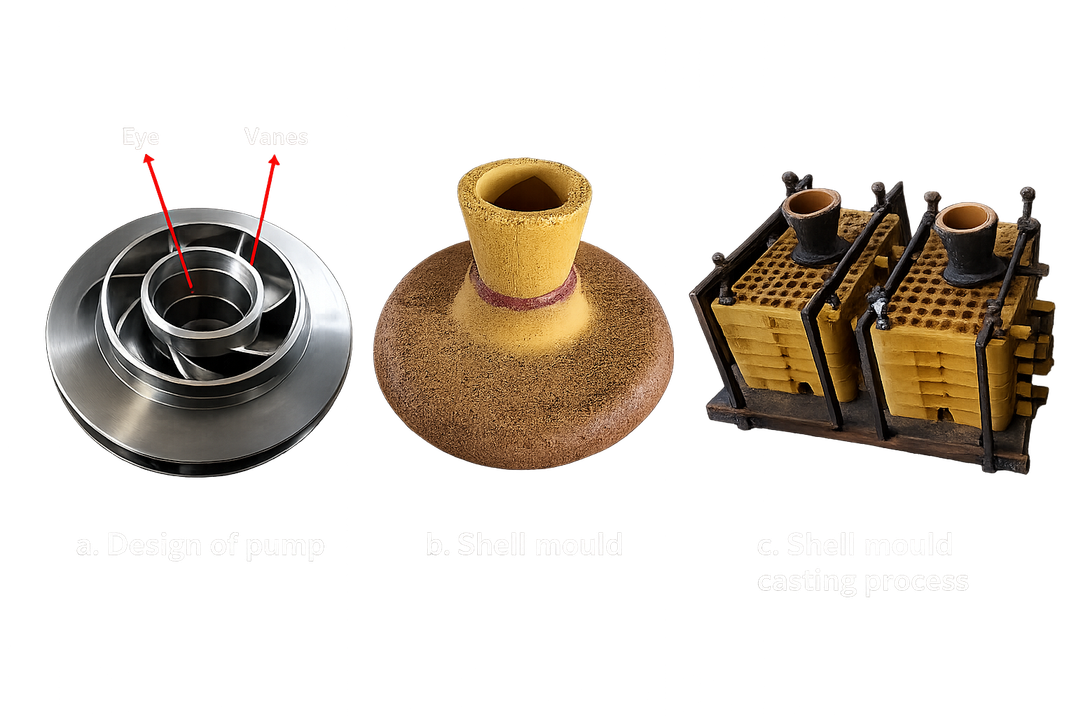
\includegraphics[width=\linewidth]{image3.png}
        \caption{Moule carapace assemble et serre dans son cadre, prêt a recevoir le metal en fusion.}
    \end{subfigure}\hfill
    \begin{subfigure}{0.46\textwidth}
        \centering
        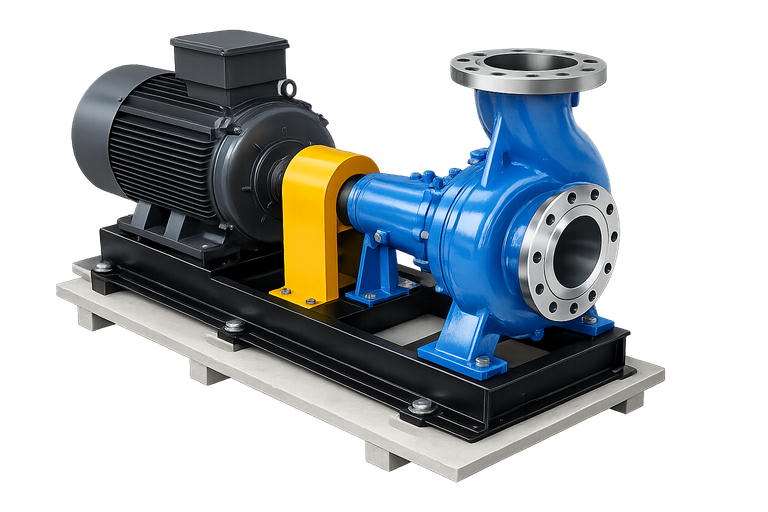
\includegraphics[width=\linewidth]{image4.png}
        \caption{Phase de coulee~: le metal liquide est verse dans les moules avant solidification.}
    \end{subfigure}
    \caption{Etapes du procede de fonderie en moule carapace.}
    \label{fig:fabrication}
\end{figure}

\paragraph{Lecture de la figure~\ref{fig:fabrication}.}
La sous-figure (a) montre l'arrangement des moules carapaces serres ensemble par un cadre exterieur~: cette configuration permet de couler plusieurs pieces simultanement et d'optimiser la productivite. La sous-figure (b) illustre la phase critique de la coulee, ou la qualite finale de la piece se joue~: vitesse de coulee, temperature du metal, vitesse de refroidissement et qualite du moule sont autant de parametres susceptibles d'introduire des defauts internes ou de surface.

\section{Typologie des defauts observes}

Apres refroidissement et demoulage, certaines pieces peuvent presenter des anomalies qui les rendent impropres a l'usage. Les defauts les plus frequemment observes sur les impellers de fonderie sont les suivants~:

\begin{itemize}
    \item \textbf{Fissures (cracks).} Discontinuites lineaires, souvent fines, resultant de tensions internes lors du refroidissement, de chocs thermiques ou d'inclusions non metalliques. Tres dangereuses car elles peuvent se propager en service sous l'effet des contraintes cycliques.
    \item \textbf{Deformations geometriques.} Ecarts par rapport a la geometrie nominale (gauchissement d'une aube, mauvaise concentricite). Causes par un retrait differentiel pendant la solidification ou par un demoulage premature.
    \item \textbf{Bavures (flash).} Excedents de matiere aux joints du moule, dus a un serrage insuffisant ou a une pression de coulee excessive.
    \item \textbf{Porosites de surface.} Petits pores visibles a la surface, resultant de gaz emprisonnes ou de retraits localises.
\end{itemize}

La figure~\ref{fig:defauts} presente un panel representatif de ces anomalies en regard d'une piece conforme.

\begin{figure}[H]
    \centering
    \begin{subfigure}{0.22\textwidth}
        \centering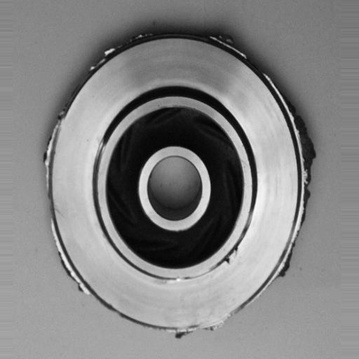
\includegraphics[width=\linewidth]{image5.jpeg}
        \caption*{\small\color{red}\textbf{Fissure}}
    \end{subfigure}\hfill
    \begin{subfigure}{0.22\textwidth}
        \centering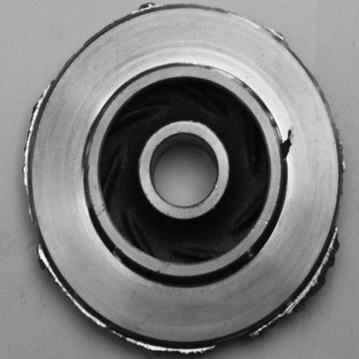
\includegraphics[width=\linewidth]{image6.jpeg}
        \caption*{\small\color{red}\textbf{Deformation}}
    \end{subfigure}\hfill
    \begin{subfigure}{0.22\textwidth}
        \centering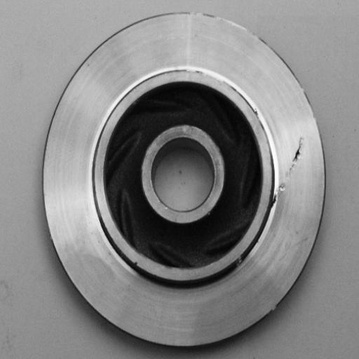
\includegraphics[width=\linewidth]{image7.jpeg}
        \caption*{\small\color{red}\textbf{Bavure}}
    \end{subfigure}\hfill
    \begin{subfigure}{0.22\textwidth}
        \centering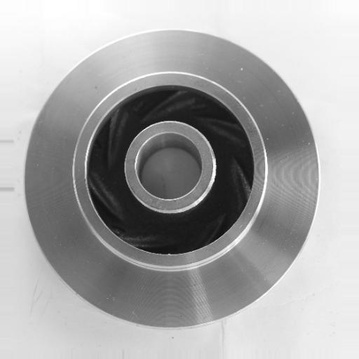
\includegraphics[width=\linewidth]{image8.jpeg}
        \caption*{\small\color{ForestGreen}\textbf{Piece normale}}
    \end{subfigure}
    \caption{Exemples typiques de defauts compares a une piece conforme.}
    \label{fig:defauts}
\end{figure}

\paragraph{Lecture de la figure~\ref{fig:defauts}.}
Cette planche illustre la diversite morphologique des anomalies. La fissure (a) est lineaire et tres locale, exigeant une resolution suffisante pour etre detectee. La deformation (b) modifie la geometrie globale de la piece, ce qui en fait un defaut detectable a basse frequence spatiale. La bavure (c) est un excedent de matiere localisee au bord. Enfin, la piece conforme (d) sert de reference visuelle a notre modele. \textbf{Cette diversite explique pourquoi un simple traitement d'image classique echoue~: les defauts n'ont ni la meme echelle, ni la meme texture, ni la meme localisation.} Seul un modele d'apprentissage profond, capable d'apprendre simultanement plusieurs niveaux d'abstraction visuelle, peut esperer detecter cette variete de cas.

\section{Objectif specifique du projet}

\begin{infobox}[title=Formulation operationnelle]
Concevoir un \textbf{classifieur binaire} prenant en entree une image numerique d'impeller et produisant en sortie une etiquette $\hat{y} \in \{\texttt{def\_front},\ \texttt{ok\_front}\}$ accompagnee d'un score de confiance $p \in [0,1]$, avec~:
\begin{itemize}
    \item un \emph{recall} sur la classe \texttt{def\_front} le plus eleve possible (priorite industrielle absolue)~;
    \item une \emph{precision} suffisante pour eviter les fausses alertes (couts de production)~;
    \item un temps d'inference compatible avec la cadence de la ligne ($<100$\,ms par piece).
\end{itemize}
\end{infobox}


% =====================================================================
%  CHAPITRE 4 - DONNEES
% =====================================================================
\chapter{Acquisition et organisation des donnees}

\section{Choix du jeu de donnees}

La construction d'un dataset specifique aux impellers de fonderie aurait necessite une campagne d'acquisition en usine, hors de portee dans le cadre de ce projet. Nous nous tournons donc vers un jeu de donnees public reconnu par la communaute~: \textbf{\emph{Casting Defect Detection}} \cite{dabhi2020casting}, cree par Ravirajsinh Dabhi et publie sur Kaggle. Ce dataset presente plusieurs avantages~:
\begin{itemize}
    \item il porte specifiquement sur des \emph{pieces de fonderie} (et non sur un domaine generique)~;
    \item les images sont prises dans des conditions \emph{realistes} d'eclairage et d'angle de vue~;
    \item il distingue explicitement deux classes (\texttt{def\_front} et \texttt{ok\_front}) representant un cas typique de classification binaire industrielle~;
    \item il propose deja une partition \emph{train/validation/test}, garantissant la comparabilite avec d'autres travaux.
\end{itemize}

\section{Description du dataset}

Le dataset \emph{Casting Defect Detection} contient des images en niveaux de gris ou couleur (selon la version) prises a la vue frontale (\emph{front}) de pieces de fonderie. Il est organise en deux classes binaires~:

\begin{itemize}
    \item \texttt{def\_front}~: pieces presentant un defaut visible (fissure, deformation, bavure, porosite).
    \item \texttt{ok\_front}~: pieces conformes aux specifications.
\end{itemize}

La figure~\ref{fig:dataset} presente un apercu visuel du dataset.

\begin{figure}[H]
    \centering
    
\includegraphics[width=0.92\textwidth]{image11.png}
    \caption{Apercu visuel du dataset \emph{Casting Defect Detection} (Kaggle).}
    \label{fig:dataset}
\end{figure}

\paragraph{Lecture de la figure~\ref{fig:dataset}.}
On observe que les images partagent une mise en cadre standardisee~: la piece est centree, prise sous un eclairage relativement uniforme et a une distance constante. Cette homogeneite est un atout pour l'apprentissage, mais elle constitue aussi une \emph{limitation}~: un modele entraine sur ces images ne generalisera pas necessairement a des conditions d'usine differentes (angles obliques, eclairages non controles). Cette consideration sera reprise dans la discussion finale.

\section{Repartition train / validation / test}

Le dataset est partitionne en trois sous-ensembles disjoints selon la strategie classique \textbf{80/10/10}~:

\begin{table}[H]
\centering
\begin{tabular}{lcc}
\toprule
\textbf{Ensemble} & \textbf{Proportion} & \textbf{Role} \\
\midrule
Train       & 80\,\% & Apprentissage des parametres du modele \\
Validation  & 10\,\% & Reglage des hyperparametres / \emph{early stopping} \\
Test        & 10\,\% & Evaluation finale (jamais vu durant l'apprentissage) \\
\bottomrule
\end{tabular}
\caption{Repartition train/validation/test du dataset.}
\label{tab:split}
\end{table}

\paragraph{Justification.} Cette partition presente trois proprietes essentielles~:
\begin{enumerate}
    \item \textbf{Disjonction stricte}~: aucune image n'appartient simultanement a deux ensembles. Cela garantit que les performances mesurees sur le test reflètent une vraie capacite de \emph{generalisation}.
    \item \textbf{Stratification}~: la proportion des classes est preservee dans chaque sous-ensemble, evitant les biais d'echantillonnage.
    \item \textbf{Reproductibilite}~: la partition est fixee par l'auteur du dataset, ce qui permet la comparaison directe entre etudes utilisant ce meme dataset.
\end{enumerate}

\section{Volumes et desequilibre des classes}

Le dataset compte environ \textbf{6\,600 images d'entrainement}, et l'ensemble de test final regroupe \textbf{715 images} (453 defectueuses, 262 conformes). On observe ainsi un leger desequilibre, avec environ \textbf{63\,\% de pieces defectueuses} contre \textbf{37\,\% de pieces conformes}. Ce desequilibre, bien que modere, justifie pleinement la mise en place d'un mecanisme de \textbf{ponderation des classes} qui sera detaille dans le chapitre suivant.

\begin{warnbox}[title=Pourquoi le desequilibre est-il un probleme?]
En l'absence de correction, un modele entraine sur un dataset desequilibre tend a apprendre la \emph{distribution prior} des classes plutot que la separation reelle entre les classes. Dans notre cas, un modele \og naif \fg\ pourrait predire systematiquement \texttt{def\_front} et atteindre $\sim 63\%$ d'\emph{accuracy} sans rien avoir appris du contenu des images~! Ce piege est fondamental et doit etre adresse explicitement.
\end{warnbox}

% =====================================================================
%  CHAPITRE 5 - PRETRAITEMENT
% =====================================================================
\chapter{Pretraitement des images}

\section{Philosophie generale du pipeline}

La phase de pretraitement est l'une des plus determinantes en apprentissage profond applique a la vision~: elle conditionne directement la \emph{capacite de generalisation} du modele final. Notre pipeline est concu autour de quatre principes directeurs~:

\begin{description}
    \item[Reproductibilite.] Toutes les sources d'aleatoire (Python, NumPy, frameworks) sont initialisees par une graine globale unique \texttt{SEED~=~42}. Une experience peut donc etre reproduite a l'identique a partir du meme code et des memes donnees.
    \item[Modularite.] Les transformations sont implementees comme des fonctions independantes, recombinables, reutilisables.
    \item[Portabilite.] Le pipeline est implemente \textbf{en double version} (\textsc{TensorFlow} et \textsc{PyTorch}), validant ainsi la robustesse de la conception.
    \item[Performance.] Utilisation systematique du parallelisme (\texttt{tf.data.AUTOTUNE} ou \texttt{num\_workers}) et du \emph{prefetching} pour saturer le \gls{gpu}.
\end{description}

% ------ TENSORFLOW PIPELINE ------
\section{Vue d'ensemble du pipeline TensorFlow (10 sections)}

L'implementation \textsc{TensorFlow} est structuree en \textbf{dix sections fonctionnelles} successives, illustrees par le bandeau de la figure~\ref{fig:tfbanner}.

\begin{figure}[H]
    \centering
    
\includegraphics[width=0.95\textwidth]{image12.jpeg}
    \caption{Bandeau de presentation du pipeline de pretraitement TensorFlow.}
    \label{fig:tfbanner}
\end{figure}

\paragraph{Lecture de la figure~\ref{fig:tfbanner}.}
Ce bandeau, utilise comme separateur visuel dans le notebook, marque l'entree dans la partie \textsc{TensorFlow} du pipeline. Il symbolise la chaine de transformations que chaque image traversera, depuis sa lecture brute sur le disque jusqu'a son arrivee comme tenseur normalise dans le modele.

Les dix sections de cette chaine sont les suivantes~:
\begin{enumerate}
    \item \textbf{Reproductibilite}~: \texttt{SEED = 42} (random, NumPy, TensorFlow).
    \item \textbf{Detection GPU/CPU}~: \texttt{tf.config.list\_physical\_devices()}.
    \item \textbf{Color Balancing}~: White Balance, Histogram Equalization, Channel Shuffle.
    \item \textbf{Normalisation ImageNet}~: $\mu = [0.485,0.456,0.406]$, $\sigma=[0.229,0.224,0.225]$.
    \item \textbf{Pipeline Train}~: crop $224\times224$, flips, rotations, jitter.
    \item \textbf{Pipeline Eval}~: \emph{center crop} deterministe + white balance.
    \item \textbf{Chargement}~: \texttt{image\_dataset\_from\_directory} pour train/val/test.
    \item \textbf{Class Weights}~: equivalent du \texttt{WeightedRandomSampler} de PyTorch.
    \item \textbf{Pipelines tf.data}~: \texttt{.map()} $\to$ \texttt{.batch()} $\to$ \texttt{.prefetch(AUTOTUNE)}.
    \item \textbf{Configuration}~: export JSON, sanity check, visualisation.
\end{enumerate}

\subsection{Reproductibilite et detection du \emph{device}}

Pour garantir la reproductibilite, toutes les sources d'aleatoire sont fixees a une meme graine~:

\begin{lstlisting}[caption={Initialisation reproductible et detection automatique du device.}]
SEED = 42
random.seed(SEED)
np.random.seed(SEED)
tf.random.set_seed(SEED)

gpus = tf.config.list_physical_devices("GPU")
DEVICE = "GPU" if gpus else "CPU"
if gpus:
    for gpu in gpus:
        tf.config.experimental.set_memory_growth(gpu, True)
\end{lstlisting}

\paragraph{Commentaire.}
L'option \texttt{set\_memory\_growth} est essentielle dans les environnements partages comme Google Colab~: elle indique a TensorFlow de n'allouer la memoire GPU qu'au fur et a mesure des besoins, plutot que de reserver l'integralite de la VRAM des l'initialisation. Cela evite les erreurs \texttt{Out-Of-Memory} lors de l'execution simultanee de plusieurs notebooks.

\paragraph{Hyperparametres globaux.}
Le tableau~\ref{tab:hyperparams} recapitule les constantes globales partagees par tous les notebooks du projet.

\begin{table}[H]
\centering
\begin{tabular}{lll}
\toprule
\textbf{Constante} & \textbf{Valeur} & \textbf{Role} \\
\midrule
\texttt{IMG\_SIZE}    & 224                          & Cote image (carree) \\
\texttt{BATCH\_SIZE}  & 32                           & Images par batch \\
\texttt{NUM\_CLASSES} & 2                            & \emph{defect} / \emph{ok\_front} \\
\texttt{MEAN}         & $[0.485, 0.456, 0.406]$      & Moyenne ImageNet (R/G/B) \\
\texttt{STD}          & $[0.229, 0.224, 0.225]$      & Ecart-type ImageNet (R/G/B) \\
\texttt{AUTOTUNE}     & \texttt{tf.data.AUTOTUNE}    & Parallelisme automatique \\
\bottomrule
\end{tabular}
\caption{Constantes globales partagees par tous les notebooks.}
\label{tab:hyperparams}
\end{table}

\subsection{Color balancing : compatibilite \emph{graph} TensorFlow}

Les images industrielles souffrent souvent de \emph{dominantes colorees} liees aux conditions d'eclairage (lumieres jaunatres ou bleuatres des ateliers). Pour rendre le modele robuste a ces variations, nous mettons en place trois transformations stochastiques de \emph{color balancing}~:

\begin{description}
    \item[Gray-World White Balance ($p=0{,}5$).] Sous l'hypothese \emph{Gray-World} (la moyenne d'une scene naturelle tend vers le gris), on normalise chaque canal par sa moyenne, puis on applique un facteur d'echelle borne dans $[0{,}5\,;\,2{,}0]$ pour eviter la sur-exposition. Implementee nativement avec \texttt{tf.cond}.
    \item[Histogram Equalization ($p=0{,}3$).] Egalise l'histogramme canal par canal via \texttt{PIL.ImageOps.equalize}, encapsulee dans \texttt{tf.py\_function}. Fait ressortir les defauts subtils dans les zones peu contrastees.
    \item[Channel Shuffle ($p=0{,}15$).] Permute aleatoirement l'ordre des canaux RGB ($6$ permutations possibles), pour rendre le modele \emph{robuste aux derives de balance des couleurs} et l'empecher d'apprendre des correlations arbitraires entre teinte et classe.
\end{description}

\begin{lstlisting}[caption={Implementation du Gray-World White Balance.}]
means = tf.reduce_mean(image, axis=[0, 1])
global_mean = tf.reduce_mean(means)
scale = global_mean / means              # (3,)
scale = tf.clip_by_value(scale, 0.5, 2.0)
return tf.clip_by_value(image * scale, 0., 1.)
\end{lstlisting}

\paragraph{Commentaire.}
Le clamp $[0.5, 2.0]$ est crucial~: sans lui, des images fortement saturees dans un canal pourraient produire des facteurs d'echelle extremes qui detruiraient l'information. Cette borne pragmatique est fixee empiriquement.

\subsection{Normalisation ImageNet}

La normalisation ImageNet aligne la distribution statistique de nos images sur celle attendue par les backbones pre-entraines~:

\begin{equation}
\hat{x} = \frac{x - \mu}{\sigma}, \qquad
\mu = \begin{pmatrix}0.485\\0.456\\0.406\end{pmatrix}, \quad
\sigma = \begin{pmatrix}0.229\\0.224\\0.225\end{pmatrix}
\label{eq:imagenet}
\end{equation}

L'equation~\eqref{eq:imagenet} centre chaque canal sur la moyenne ImageNet et le reduit par son ecart-type. Cette etape est \emph{indispensable} pour le \emph{Transfer Learning}~: les filtres pre-entraines de \textsc{EfficientNetB0} ont ete optimises sur des entrees ainsi normalisees, et tout ecart de distribution entrainerait une chute drastique de performance.

\subsection{Comparaison train vs eval}

Une regle absolue en apprentissage profond~: \textbf{l'augmentation de donnees ne s'applique qu'a l'entrainement}. Le tableau~\ref{tab:traineval} compare les transformations appliquees dans chaque mode.

\begin{table}[H]
\centering\small
\begin{tabular}{lll}
\toprule
\textbf{Operation} & \texttt{preprocess\_train} & \texttt{preprocess\_eval} \\
\midrule
Resize         & $256\times256$             & $256\times256$ \\
Crop           & random $224\times224$      & center crop $224\times224$ \\
Flips          & H + V                      & --- \\
Rotation       & $\pm 180^\circ$ (\texttt{tfa})  & --- \\
Color balance  & stochastique               & deterministe ($p=1$) \\
Color jitter   & brightness/contrast/sat/hue & --- \\
Grayscale      & $p=0{,}1$                  & --- \\
Normalisation  & ImageNet                   & ImageNet \\
\bottomrule
\end{tabular}
\caption{Comparaison des transformations \emph{train} vs \emph{eval}.}
\label{tab:traineval}
\end{table}

\paragraph{Pourquoi cette dissymetrie?}
En entrainement, on cherche a \emph{augmenter virtuellement} la taille du dataset par des transformations stochastiques, ce qui force le modele a apprendre des representations invariantes. En evaluation, au contraire, on veut une mesure \emph{deterministe} et \emph{reproductible} des performances~: appliquer des transformations aleatoires biaiserait la mesure. Le seul \emph{color balancing} eval applique est le White Balance avec $p=1$, deterministe par construction.

\subsection{Chargement et ponderation des classes}

\begin{lstlisting}[caption={Chargement \texttt{tf.data} et calcul des poids de classes.}]
def _load_raw(directory, shuffle):
    return tf.keras.utils.image_dataset_from_directory(
        directory, labels="inferred", label_mode="int",
        color_mode="rgb", batch_size=None,
        image_size=(256, 256), shuffle=shuffle, seed=SEED,
    )

raw_train = _load_raw(TRAIN_DIR, shuffle=True)
raw_val   = _load_raw(VAL_DIR,   shuffle=False)
raw_test  = _load_raw(TEST_DIR,  shuffle=False)

all_labels   = np.array([lbl.numpy() for _, lbl in raw_train])
class_counts = np.bincount(all_labels, minlength=NUM_CLASSES)
total        = len(all_labels)
class_weights = {
    i: float(total) / (NUM_CLASSES * int(count))
    for i, count in enumerate(class_counts)
}
\end{lstlisting}

La ponderation suit la formule classique \emph{inverse frequency weighting}~:
\begin{equation}
w_i \;=\; \frac{N_\text{total}}{N_\text{classes}\,\cdot\,n_i}
\label{eq:classweight}
\end{equation}
Cette formule donne un poids superieur a la classe minoritaire (\texttt{ok\_front}) afin que le modele consacre proportionnellement plus d'attention aux echantillons rares lors du calcul de la fonction de perte.

\subsection{Composition finale des datasets}

\begin{lstlisting}[caption={Composition finale~: \texttt{.map()} -> \texttt{.batch()} -> \texttt{.prefetch()}.}]
train_dataset = (raw_train
    .map(preprocess_train, num_parallel_calls=AUTOTUNE)
    .batch(BATCH_SIZE, drop_remainder=True)
    .prefetch(AUTOTUNE))

val_dataset = (raw_val
    .map(preprocess_eval,  num_parallel_calls=AUTOTUNE)
    .batch(BATCH_SIZE).prefetch(AUTOTUNE))

test_dataset = (raw_test
    .map(preprocess_eval,  num_parallel_calls=AUTOTUNE)
    .batch(BATCH_SIZE).prefetch(AUTOTUNE))
\end{lstlisting}

\paragraph{Commentaire.}
L'ordre \texttt{.map()} $\to$ \texttt{.batch()} $\to$ \texttt{.prefetch()} est crucial. \texttt{.map()} applique la transformation a chaque image \emph{individuellement} en parallele, \texttt{.batch()} regroupe ensuite les images traitees en batches, et \texttt{.prefetch(AUTOTUNE)} permet au CPU de preparer le prochain batch pendant que le GPU traite l'actuel --- realisant ainsi un pipelining qui maximise l'utilisation des deux unites de calcul.

\subsection{Configuration centralisee et utilitaires}

\begin{lstlisting}[caption={Export centralise de la configuration au format JSON.}]
CONFIG = {
    "img_size"     : 224,
    "batch_size"   : 32,
    "num_classes"  : 2,
    "class_names"  : ["defect", "ok_front"],
    "mean"         : [0.485, 0.456, 0.406],
    "std"          : [0.229, 0.224, 0.225],
    "class_weights": {"0": 1.12, "1": 0.90},
    "device"       : "GPU"
}
\end{lstlisting}

Quatre utilitaires complètent le module \texttt{preprocessing\_tf}~:
\begin{itemize}
    \item \texttt{sanity\_check()} --- affiche \emph{shape}, min/max/mean d'un batch.
    \item \texttt{show\_batch(ds, n=8)} --- visualise $n$ images avec leur label.
    \item \texttt{plot\_class\_distribution()} --- histogramme \emph{defect} vs \emph{ok\_front}.
    \item \texttt{compute\_mean\_std(ds, n=20)} --- moyenne et ecart-type empiriques.
\end{itemize}

La figure~\ref{fig:utils} regroupe les sorties typiques de ces quatre utilitaires.

\begin{figure}[H]
    \centering
    \begin{subfigure}{0.32\textwidth}
        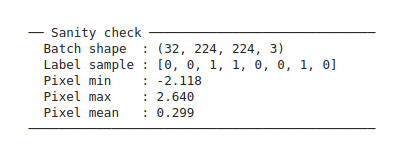
\includegraphics[width=\linewidth]{image13.png}
        \caption{Sortie de \texttt{sanity\_check()}}
    \end{subfigure}\hfill
    \begin{subfigure}{0.32\textwidth}
        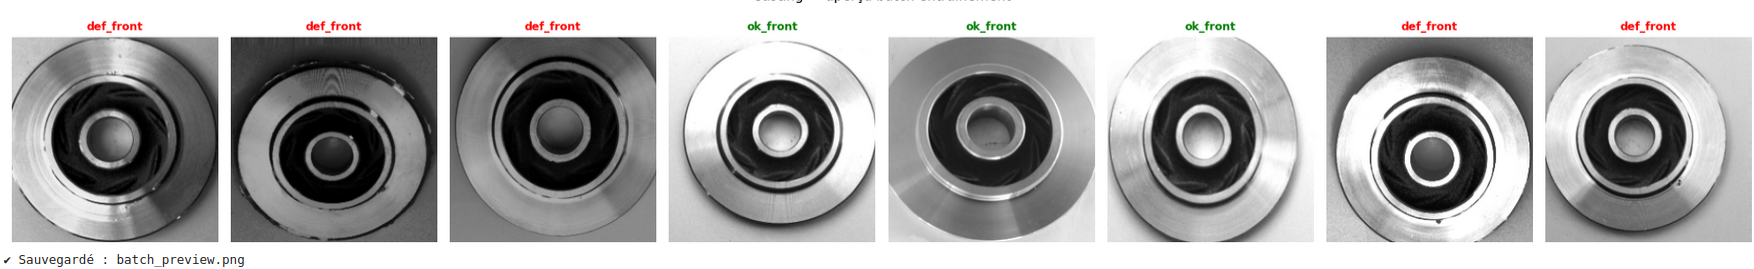
\includegraphics[width=\linewidth]{image14.png}
        \caption{Sortie de \texttt{show\_batch()}}
    \end{subfigure}\hfill
    \begin{subfigure}{0.32\textwidth}
        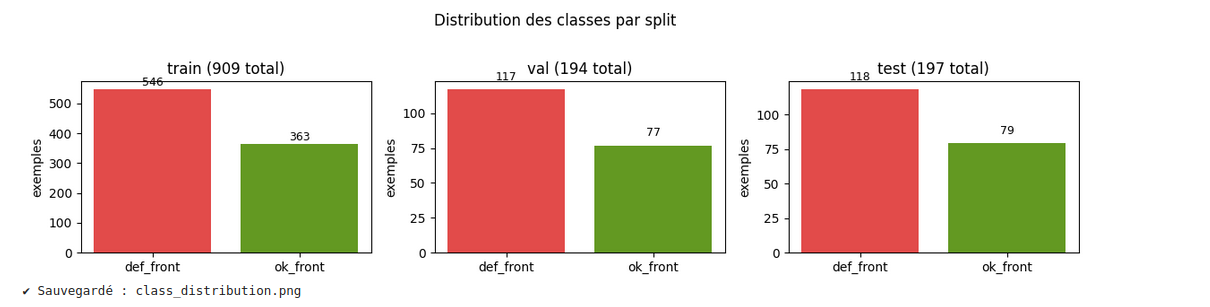
\includegraphics[width=\linewidth]{image15.png}
        \caption{Distribution des classes par split}
    \end{subfigure}
    \caption{Sorties des utilitaires de controle du pipeline.}
    \label{fig:utils}
\end{figure}

\paragraph{Lecture de la figure~\ref{fig:utils}.}
La sous-figure (a) confirme la coherence des shapes du batch ($32 \times 224 \times 224 \times 3$) ainsi que les statistiques pixel apres normalisation ($\min \approx -2.1$, $\max \approx 2.6$, $\mu \approx 0.3$) --- valeurs coherentes avec la normalisation ImageNet, ce qui valide la chaine de pretraitement. La sous-figure (b) presente un batch de 8 images apres pretraitement complet~: on y voit des pieces dans des orientations variees, traduisant l'effet des rotations et des flips. La sous-figure (c) confirme visuellement le desequilibre annonce des classes~: la barre rouge (\texttt{def\_front}) est systematiquement superieure a la verte (\texttt{ok\_front}) dans les trois splits, ce qui justifie a posteriori le mecanisme de \emph{class weighting} mis en place.

% ------ PYTORCH PIPELINE ------
\section{Pipeline equivalent en PyTorch}

Le pipeline \textsc{PyTorch} reprend les memes etapes que la version TensorFlow, mais s'appuie sur les abstractions natives de \texttt{torchvision.transforms} et un \texttt{DataLoader} avec \texttt{WeightedRandomSampler}.

\subsection{Reproductibilite et device}

\begin{lstlisting}[caption={Reproductibilite et detection automatique du device en PyTorch.}]
SEED = 42
random.seed(SEED); np.random.seed(SEED)
torch.manual_seed(SEED); torch.cuda.manual_seed_all(SEED)
torch.backends.cudnn.deterministic = True
torch.backends.cudnn.benchmark = False

DEVICE = torch.device("cuda" if torch.cuda.is_available() else "cpu")
\end{lstlisting}

\paragraph{Commentaire.}
Les options \texttt{cudnn.deterministic = True} et \texttt{cudnn.benchmark = False} forcent CUDA a utiliser des algorithmes deterministes, au prix d'une legere perte de performance. C'est un \emph{compromis assume} en faveur de la reproductibilite, particulierement important en contexte academique ou industriel ou les resultats doivent pouvoir etre reproduits a l'identique.

\subsection{Color balancing personnalise}

PyTorch ne propose pas nativement les transformations de \emph{color balancing} dont nous avons besoin~; nous les implementons donc comme des classes heritant de \texttt{torch.nn.Module}~:

\begin{itemize}
    \item \textbf{AutoWhiteBalance} ($p=0{,}5$) --- hypothese \emph{Gray-World} pour corriger les dominantes colorees des cameras industrielles.
    \item \textbf{HistogramEqualization} ($p=0{,}3$) --- fait ressortir les defauts subtils dans les zones peu contrastees.
    \item \textbf{ChannelShuffle} ($p=0{,}15$) --- permute les canaux RGB pour rendre le modele independant de la teinte de surface.
\end{itemize}

\subsection{Pipeline complet d'augmentations}

Les transformations appliquees au \emph{train} se composent comme suit~:
\begin{enumerate}
    \item \texttt{Resize(256, 256)} --- uniformisation de la taille d'entree.
    \item \texttt{RandomCrop(224)} --- recadrage aleatoire $224\times224$ pour introduire de la variabilite spatiale.
    \item \texttt{RandomHorizontalFlip(0.5)} et \texttt{RandomVerticalFlip(0.5)} --- les images industrielles n'ont pas d'orientation privilegiee.
    \item \texttt{RandomRotation(180)} --- rotations jusqu'a $\pm 180^\circ$~: invariance rotationnelle complete.
    \item \texttt{AutoWhiteBalance(0.5)}, \texttt{HistogramEqualization(0.3)}, \texttt{ChannelShuffle(0.15)} --- robustesse couleur.
    \item \texttt{ColorJitter(0.2, 0.3, 0.1, 0.02)} --- variations \emph{brightness, contrast, saturation, hue}.
    \item \texttt{RandomAffine(translate=(0.05, 0.05))} --- translations $\pm5\%$~: robustesse aux decalages de cadrage.
    \item \texttt{RandomGrayscale(0.1)} --- 10\% des images converties en niveaux de gris.
    \item \texttt{GaussianBlur(3)} --- flou leger~: robustesse au bruit de capteur.
    \item \texttt{ToTensor()} et \texttt{Normalize($\mu, \sigma$)} (ImageNet).
\end{enumerate}

\subsection{Gestion du desequilibre des classes}

Le dataset presente un leger desequilibre ($\sim 65\%$ \texttt{def\_front} vs $\sim 35\%$ \texttt{ok\_front}). Sans correction, le modele apprendrait a toujours predire la classe majoritaire. Nous utilisons un \texttt{WeightedRandomSampler}~:

\begin{lstlisting}[caption={Ponderation inverse-frequence des echantillons.}]
class_counts   = torch.bincount(targets)
class_weights  = 1.0 / class_counts
sample_weights = class_weights[targets]
sampler = WeightedRandomSampler(
    sample_weights, num_samples=len(sample_weights),
    replacement=True
)
\end{lstlisting}

\paragraph{Commentaire.}
L'option \texttt{replacement=True} est essentielle~: sans elle, les echantillons de la classe minoritaire seraient epuises avant ceux de la classe majoritaire. Avec replacement, chaque epoque tire $N$ echantillons au sort selon la distribution ponderee, garantissant une exposition equilibree du modele aux deux classes.

\subsection{DataLoaders et utilitaires}

Le tableau~\ref{tab:loaders} resume la configuration des trois \texttt{DataLoaders}.

\begin{table}[H]
\centering
\begin{tabular}{lcccc}
\toprule
\textbf{Loader} & \texttt{batch\_size} & \texttt{shuffle} & \textbf{Sampler} & \texttt{pin\_memory} \\
\midrule
\texttt{train\_loader} & 32 & --- & WeightedRandom & si CUDA \\
\texttt{val\_loader}   & 32 & False & --- & si CUDA \\
\texttt{test\_loader}  & 32 & False & --- & si CUDA \\
\bottomrule
\end{tabular}
\caption{Configuration des trois \texttt{DataLoaders} PyTorch.}
\label{tab:loaders}
\end{table}

\paragraph{Pourquoi \texttt{pin\_memory=True}?}
L'option \texttt{pin\_memory} alloue les tenseurs dans une zone memoire CPU \og pinnee \fg, accelerant le transfert vers le GPU via DMA asynchrone. Le gain peut atteindre 30\% sur les transferts CPU-GPU, ce qui est significatif lorsque le bottleneck du training est le chargement des donnees.


% =====================================================================
%  CHAPITRE 6 - MODELISATION
% =====================================================================
\chapter{Modelisation et experimentations}

Dans ce chapitre, nous developpons et comparons \textbf{trois architectures de classification} suivant une demarche progressive~: (i) un Perceptron Multi-Couches (\gls{mlp}) servant de baseline, (ii) un Reseau de Neurones Convolutif (\gls{cnn}) entraine de zero, et (iii) un modele de \emph{Transfer Learning} fonde sur \textsc{EfficientNetB0}. Cette demarche permet de mettre en evidence, de maniere empirique et pedagogique, l'apport specifique de chaque famille architecturale.

% --------------------------------------------------------- MLP
\section{Modele 1 : Perceptron Multi-Couches (MLP)}

\subsection{Motivation}

Le \gls{mlp} constitue le modele de neurones le plus elementaire capable d'apprentissage supervise non-lineaire. Il sert ici de \textbf{baseline}~: a la fois comme reference de performance \emph{minimale} et comme pretexte pedagogique pour mettre en evidence les limites des reseaux \emph{denses} face aux donnees structurees comme les images.

\subsection{Representation des donnees : le Flatten}

Les images d'entree sont des tenseurs $224 \times 224 \times 3$ (hauteur $\times$ largeur $\times$ canaux). Or, un MLP ne sait traiter que des \emph{vecteurs unidimensionnels}~: il faut donc \emph{aplatir} l'image, operation realisee par la couche \texttt{Flatten}~:

\begin{equation}
(224 \times 224 \times 3) \;\longrightarrow\; \mathbb{R}^{150\,528}
\label{eq:flatten}
\end{equation}

\begin{figure}[H]
    \centering
    \begin{subfigure}{0.34\textwidth}
        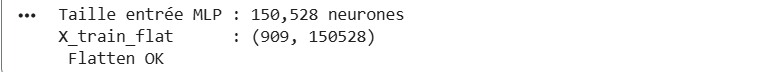
\includegraphics[width=\linewidth]{image17.png}
        \caption{Image d'entree 3D ($224\times224\times3$)}
    \end{subfigure}\hfill
    \begin{subfigure}{0.62\textwidth}
        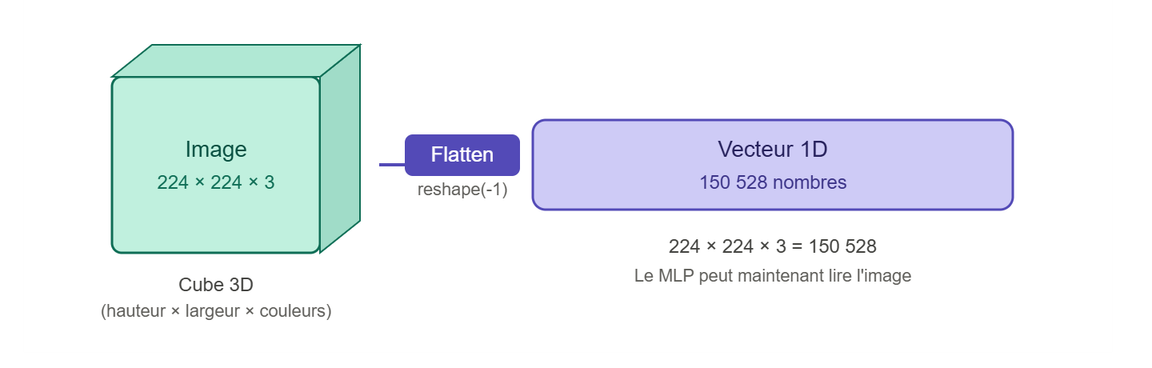
\includegraphics[width=\linewidth]{image18.png}
        \caption{Vectorisation par \texttt{Flatten} en $\mathbb{R}^{150\,528}$}
    \end{subfigure}
    \caption{Aplatissement (\emph{Flatten}) d'une image en vecteur 1D.}
    \label{fig:flatten}
\end{figure}

\paragraph{Lecture de la figure~\ref{fig:flatten}.}
La sous-figure (a) represente l'image dans sa structure naturelle 3D, ou la \emph{proximite spatiale} entre pixels traduit une realite physique~: deux pixels voisins horizontalement ou verticalement appartiennent typiquement a la meme region (meme aube, meme bord). La sous-figure (b) illustre la transformation \texttt{Flatten}, qui \emph{lineairise} ces 150\,528 valeurs sans aucune notion d'adjacence. \textbf{C'est la limite fondamentale du MLP applique aux images}~: deux pixels voisins en 2D peuvent se retrouver tres eloignes dans le vecteur 1D, ce qui empeche le reseau de tirer parti de la structure spatiale.

\subsection{Architecture du MLP}

\begin{infobox}[title=Architecture du MLP]
\textbf{Entree}~: $150\,528$ neurones\\
$\to$ Dense(512) + BatchNorm + ReLU + Dropout(0.4)\\
$\to$ Dense(256) + BatchNorm + ReLU + Dropout(0.4)\\
$\to$ Dense(128) + BatchNorm + ReLU + Dropout(0.3)\\
$\to$ Dense(2) + \textbf{Softmax}\quad ($\to$ \texttt{def\_front} / \texttt{ok\_front})
\end{infobox}

La figure~\ref{fig:mlparch} represente schematiquement cette architecture.

\begin{figure}[H]
    \centering
    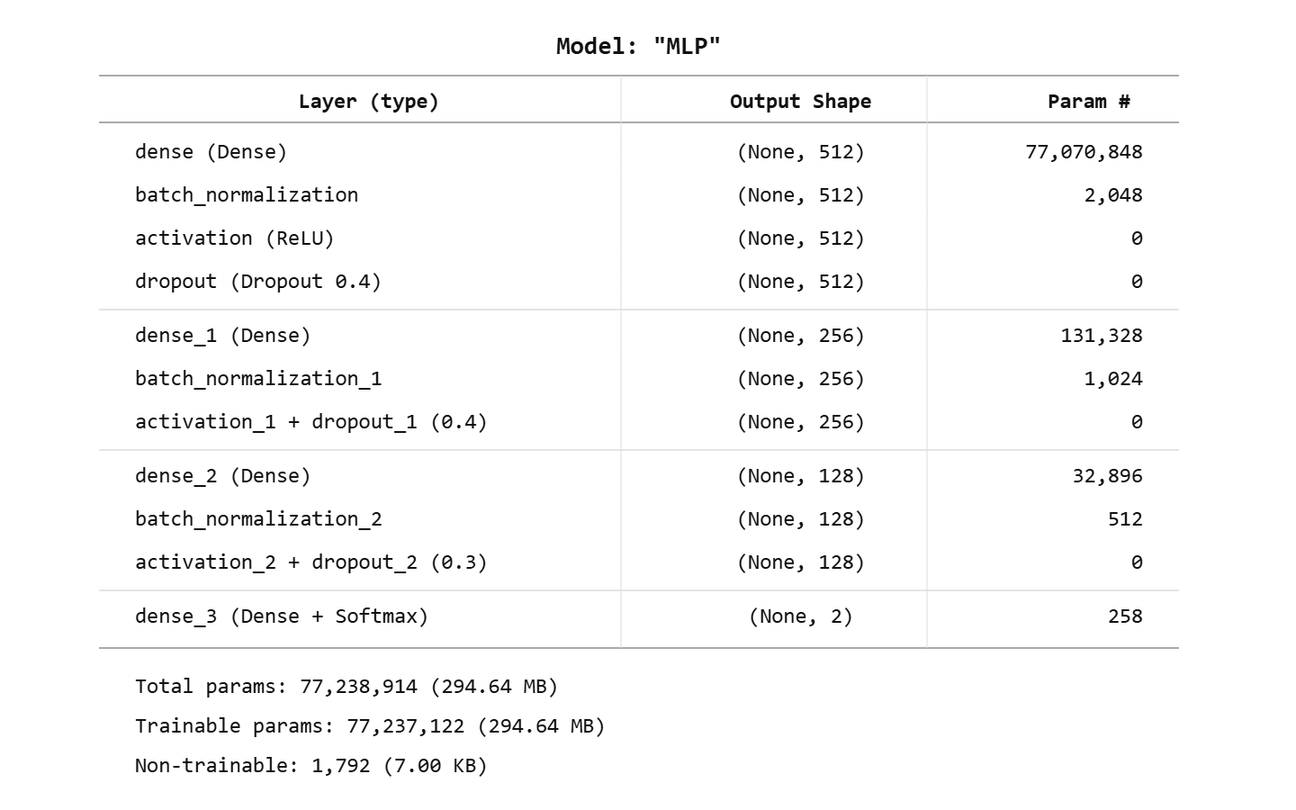
\includegraphics[width=0.85\textwidth]{image19.png}
    \caption{Schema global de l'architecture MLP.}
    \label{fig:mlparch}
\end{figure}

\paragraph{Lecture de la figure~\ref{fig:mlparch}.}
Le reseau enchaine trois blocs denses dont la dimension decroit progressivement ($512 \to 256 \to 128$). Cette decroissance, classique en architecture neuronale, joue le role d'un \emph{compresseur d'information}~: le reseau doit progressivement \emph{filtrer} l'information pertinente parmi les 150\,528 features brutes. La sortie est une couche dense de 2 neurones suivie d'une fonction \emph{Softmax} qui produit une distribution de probabilite sur les deux classes.

\subsection{Mecanismes de regularisation}

Trois mecanismes de regularisation sont integres pour limiter le sur-apprentissage~:

\begin{itemize}
    \item \textbf{Batch Normalization} \cite{ioffe2015}~: normalise les activations intermediaires sur le batch, stabilisant et accelerant l'apprentissage. Mathematiquement, pour une activation $x$ d'un mini-batch~:
    \begin{equation}
    \hat{x} = \frac{x - \mu_B}{\sqrt{\sigma_B^2 + \epsilon}}, \quad y = \gamma \hat{x} + \beta
    \end{equation}
    ou $\gamma, \beta$ sont des parametres appris.
    \item \textbf{Dropout} \cite{srivastava2014}~: a chaque iteration d'entrainement, une fraction $p$ des neurones est aleatoirement desactivee. Cela force le reseau a apprendre des representations \emph{redondantes} et l'empeche de trop dependre d'un sous-ensemble de neurones.
    \item \textbf{Early Stopping (patience = 7)}~: arret automatique de l'entrainement si la perte de validation cesse de diminuer pendant 7 epoques consecutives. Sauvegarde le meilleur modele observe.
    \item \textbf{ReduceLROnPlateau}~: divise le \emph{learning rate} par 2 si la perte stagne, permettant un \emph{fine-tuning} progressif.
\end{itemize}

\subsection{Resultats du MLP}

Le modele est entraine pendant un maximum de 30 epoques avec optimiseur Adam (LR initial = 1e-3) et perte \emph{categorical crossentropy}. Les courbes d'apprentissage et la matrice de confusion finale sont presentees figure~\ref{fig:mlpresults}.

\begin{figure}[H]
    \centering
    \begin{subfigure}{0.48\textwidth}
        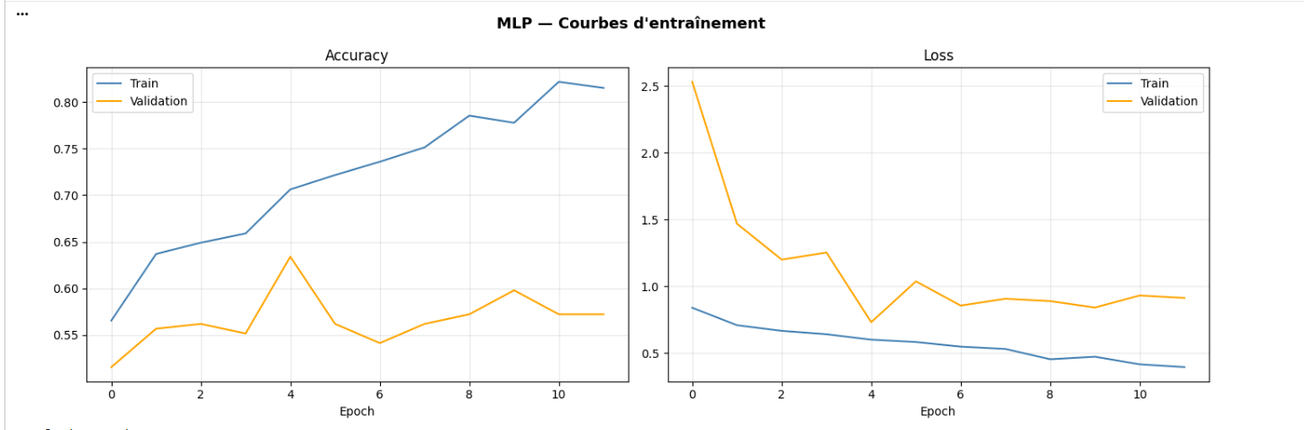
\includegraphics[width=\linewidth]{image22.png}
        \caption{Courbes de \emph{loss} et \emph{accuracy} (train / val)}
    \end{subfigure}\hfill
    \begin{subfigure}{0.42\textwidth}
        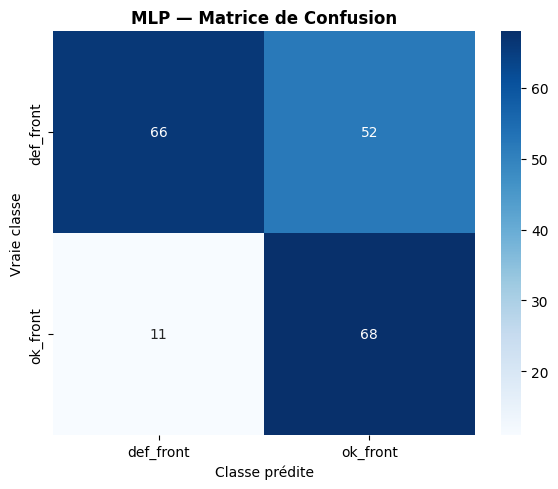
\includegraphics[width=\linewidth]{image24.png}
        \caption{Matrice de confusion}
    \end{subfigure}
    \caption{Performance du MLP sur le jeu de test.}
    \label{fig:mlpresults}
\end{figure}

\paragraph{Lecture de la figure~\ref{fig:mlpresults}.}
La sous-figure (a) montre que l'\emph{accuracy} de train et de validation evoluent de maniere proche, plafonnant rapidement autour de $\sim 70\%$. La perte (\emph{loss}) decroit puis se stabilise. L'absence d'ecart marque entre train et validation indique \textbf{l'absence de sur-apprentissage}~: le probleme du MLP n'est pas qu'il apprend par c\oe ur ses donnees, mais qu'il n'est \emph{intrinsequement pas capable} d'apprendre une fonction de classification suffisamment expressive sur ce type d'entree. La sous-figure (b) confirme cette analyse~: la matrice de confusion montre des erreurs symetriquement reparties sur les deux classes (52 \texttt{def\_front} mal classees, 11 \texttt{ok\_front} mal classees), traduisant une difficulte structurelle plutot qu'un biais.

Le tableau~\ref{tab:mlpresults} synthetise les metriques finales sur le test.

\begin{table}[H]
\centering
\begin{tabular}{lc}
\toprule
\textbf{Metrique} & \textbf{Valeur} \\
\midrule
Test Loss     & $0{,}7587$ \\
Test Accuracy & $68{,}02\,\%$ \\
Precision     & $74{,}07\,\%$ \\
Recall        & $68{,}02\,\%$ \\
F1-Score      & $67{,}95\,\%$ \\
Epochs entraines & $12 / 30$ (early stopping declenche) \\
\bottomrule
\end{tabular}
\caption{Resultats du MLP sur l'ensemble de test.}
\label{tab:mlpresults}
\end{table}

\subsection{Analyse critique du MLP}

\begin{description}
    \item[Points forts.] Convergence rapide (12 epoques), modele simple a comprendre et a entrainer, baseline honnete pour quantifier l'apport des architectures suivantes.
    \item[Limites.] La couche \texttt{Flatten} \textbf{detruit la structure spatiale}~: les pixels voisins perdent leur lien, le modele ne peut pas apprendre de \emph{textures} ni de \emph{contours}. De plus, le nombre colossal de parametres dans la premiere couche dense ($150\,528 \times 512 \approx 77$ millions !) est totalement disproportionne par rapport a la taille du dataset, augmentant le risque de sur-apprentissage et alourdissant inutilement le modele.
\end{description}

$\Rightarrow$ Ces limitations motivent le passage a un modele exploitant explicitement la structure 2D de l'image~: le \textbf{Reseau de Neurones Convolutif (CNN)}.

% --------------------------------------------------------- CNN
\section{Modele 2 : CNN entraine de zero}

\subsection{Principe et fondements theoriques}

Un \textbf{Reseau de Neurones Convolutif (CNN)} \cite{lecun1998} est une architecture concue specifiquement pour exploiter la structure spatiale des images. Il repose sur trois operations fondamentales~:

\begin{enumerate}
    \item \textbf{La convolution}~: un filtre (ou \emph{kernel}) de taille reduite (typiquement $3\times 3$) glisse sur l'image et calcule un produit scalaire local. Le meme filtre est applique partout (\emph{poids partages}), ce qui reduit drastiquement le nombre de parametres et confere au reseau une \emph{invariance par translation}.
    \item \textbf{Le pooling}~: reduction spatiale (\emph{max pooling} ou \emph{average pooling}) qui resume une region locale en un unique pixel, augmentant le champ receptif et reduisant la dimension.
    \item \textbf{Les non-linearites}~: typiquement \gls{relu} (Rectified Linear Unit), qui introduit la capacite de modeliser des fonctions non-lineaires complexes.
\end{enumerate}

L'empilement de ces operations construit une \emph{hierarchie de representations}~: les premieres couches detectent des contours et des couleurs, les couches intermediaires des textures et des motifs, les couches profondes des concepts semantiques.

\subsection{Architecture du CNN propose}

Notre CNN enchaine plusieurs blocs convolutifs, chacun compose d'une couche \texttt{Conv2D}, suivie de \texttt{BatchNormalization}, d'une activation \texttt{ReLU} et d'une couche \texttt{MaxPooling2D}. La figure~\ref{fig:cnnarch} illustre l'architecture globale.

\begin{figure}[H]
    \centering
    \begin{subfigure}{0.46\textwidth}
        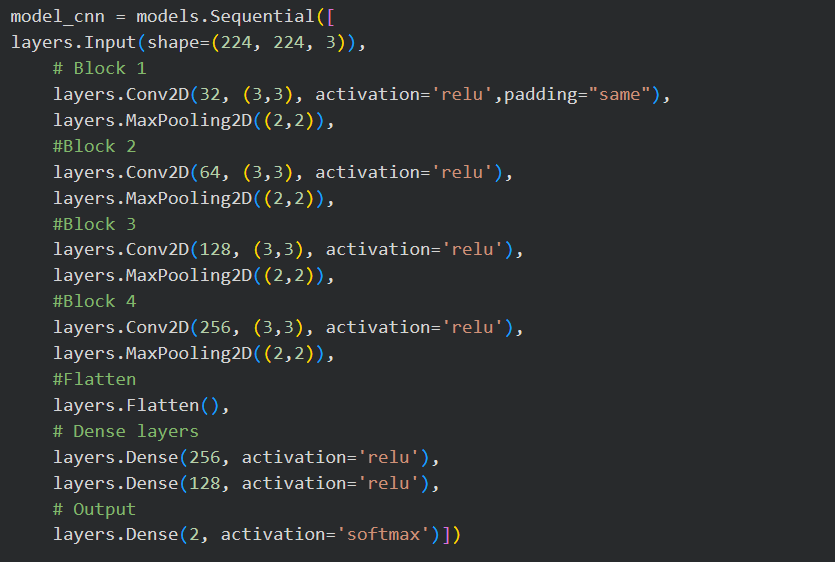
\includegraphics[width=\linewidth]{image27.png}
        \caption{Bloc convolutif elementaire}
    \end{subfigure}\hfill
    \begin{subfigure}{0.46\textwidth}
        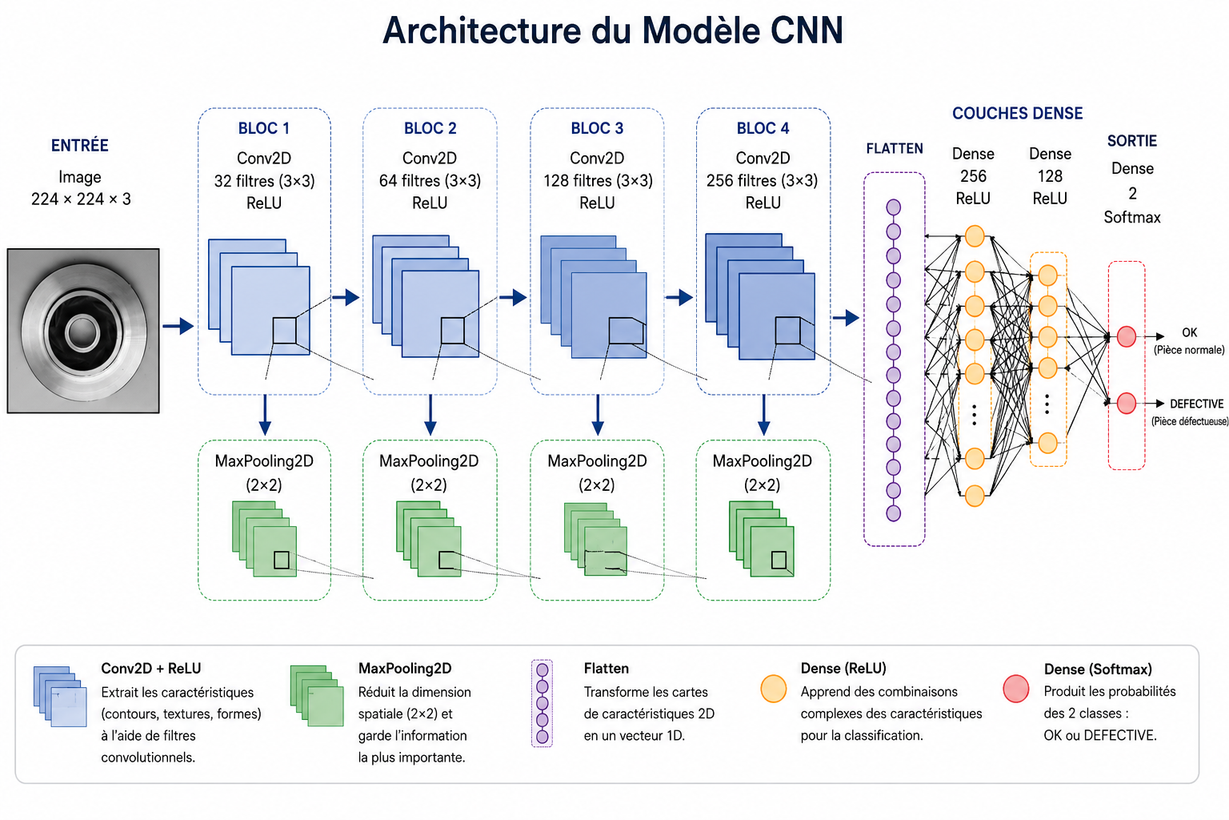
\includegraphics[width=\linewidth]{image30.png}
        \caption{Vue d'ensemble du CNN}
    \end{subfigure}
    \caption{Architecture du CNN entraine de zero.}
    \label{fig:cnnarch}
\end{figure}

\paragraph{Lecture de la figure~\ref{fig:cnnarch}.}
La sous-figure (a) presente la \emph{cellule elementaire} repetee dans le reseau~: convolution, batch norm, ReLU, pooling. C'est l'unite atomique d'extraction de caracteristiques. La sous-figure (b) montre l'agencement global~: plusieurs blocs convolutifs en serie, dont la profondeur (nombre de filtres) augmente progressivement, suivis d'un \emph{Global Average Pooling} et d'une tete de classification dense. Cette architecture pyramidale est typique des CNN et reflète la hierarchie d'abstraction visuelle evoquee plus haut.

\subsection{Compilation et regularisation}

Le modele est compile avec~:
\begin{itemize}
    \item \textbf{Optimiseur}~: \texttt{Adam} \cite{kingma2014} avec \texttt{learning\_rate=1e-3}.
    \item \textbf{Fonction de perte}~: \emph{categorical crossentropy} (formulation pour 2 classes one-hot).
    \item \textbf{Metriques}~: accuracy.
\end{itemize}

Plusieurs mecanismes de regularisation sont integres~:

\begin{figure}[H]
    \centering
    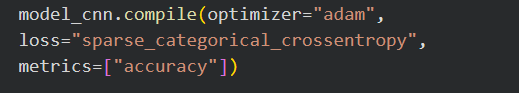
\includegraphics[width=0.7\textwidth]{image31.png}
    \caption{Compilation et configuration du CNN avec callbacks de regularisation.}
    \label{fig:cnncomp}
\end{figure}

\paragraph{Lecture de la figure~\ref{fig:cnncomp}.}
La compilation Keras revele trois mecanismes de regularisation simultanes~: l'\emph{Early Stopping} (arret si la val\_loss ne s'ameliore plus), la \emph{Batch Normalization} (deja decrite, integree dans chaque bloc convolutif) et le \emph{Dropout} (desactivation aleatoire de neurones). La combinaison de ces trois mecanismes correspond aux meilleures pratiques actuelles pour entrainer un CNN sur un dataset de taille moderee.

\subsection{Entrainement}

Le CNN est entraine pendant 30 epoques maximum, avec batch de taille 32. La figure~\ref{fig:cnntrain} montre la boucle d'entrainement et un extrait des logs Keras.

\begin{figure}[H]
    \centering
    \begin{subfigure}{0.47\textwidth}
        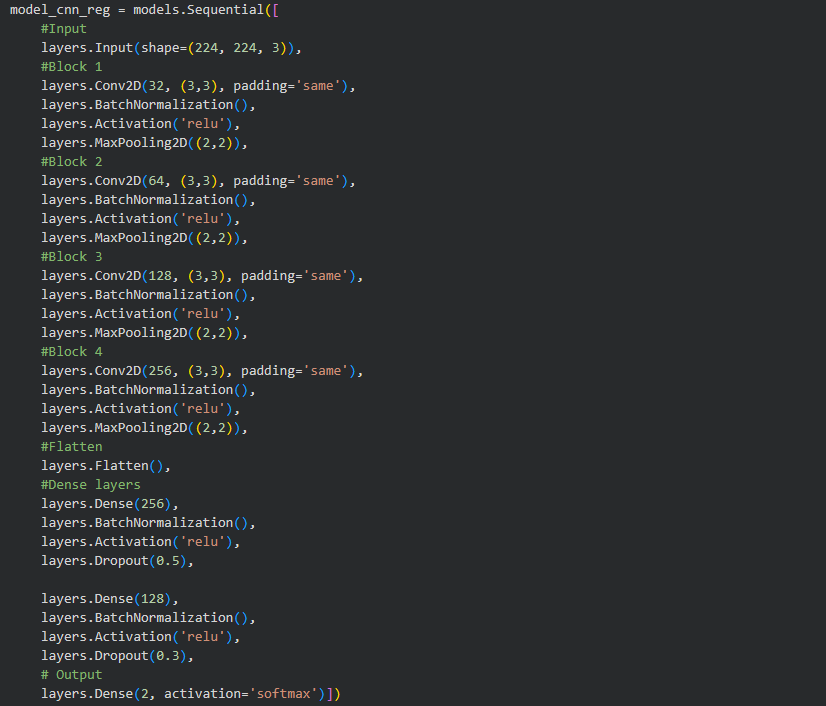
\includegraphics[width=\linewidth]{image32.png}
        \caption{Boucle d'entrainement \texttt{model.fit()}}
    \end{subfigure}\hfill
    \begin{subfigure}{0.47\textwidth}
        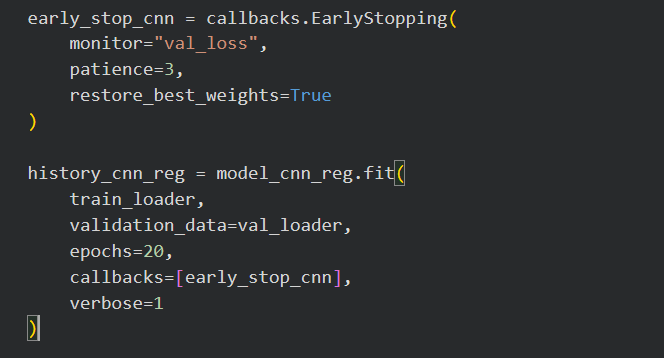
\includegraphics[width=\linewidth]{image33.png}
        \caption{Extrait des logs Keras}
    \end{subfigure}
    \caption{Entrainement du CNN sur 30 epoques.}
    \label{fig:cnntrain}
\end{figure}

\paragraph{Lecture de la figure~\ref{fig:cnntrain}.}
La sous-figure (a) montre l'appel canonique \texttt{model.fit()} avec ses parametres essentiels~: dataset d'entrainement, dataset de validation, nombre d'epoques, callbacks. La sous-figure (b) presente un extrait des logs~: on y voit les progres epoque par epoque, avec accuracy de train et accuracy de validation. Ces logs sont essentiels pour le diagnostic en temps reel du comportement du modele.

\subsection{Evaluation et diagnostic d'overfitting}

Les courbes d'apprentissage du CNN sans data augmentation revelent un comportement caracteristique illustre figure~\ref{fig:cnnoverfit}.

\begin{figure}[H]
    \centering
    \begin{subfigure}{0.47\textwidth}
        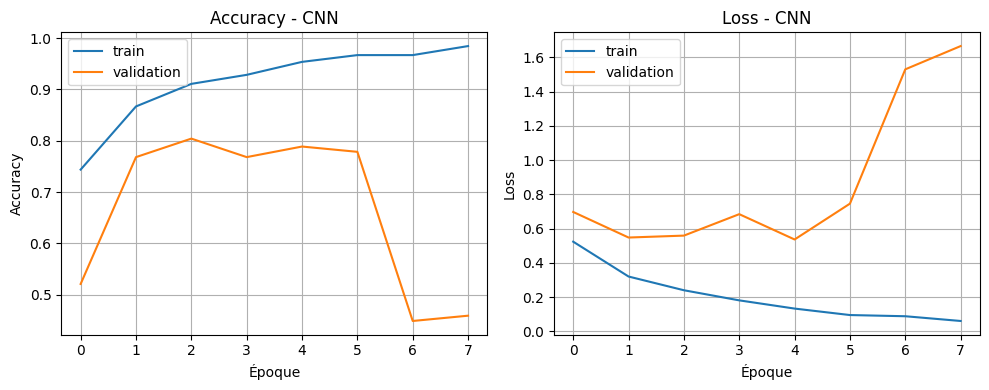
\includegraphics[width=\linewidth]{image34.png}
        \caption{\emph{Accuracy} train (bleue) vs validation (orange)}
    \end{subfigure}\hfill
    \begin{subfigure}{0.47\textwidth}
        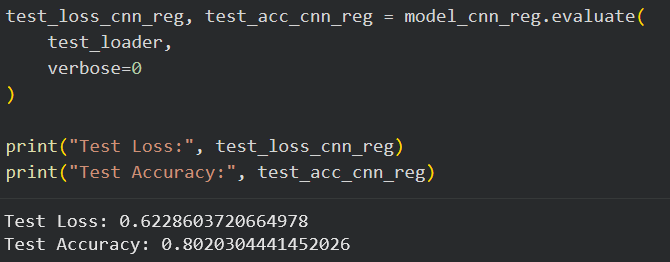
\includegraphics[width=\linewidth]{image35.png}
        \caption{\emph{Loss} train (bleue) vs validation (orange)}
    \end{subfigure}
    \caption{Courbes d'entrainement du CNN avant data augmentation~: signe clair de sur-apprentissage.}
    \label{fig:cnnoverfit}
\end{figure}

\paragraph{Lecture de la figure~\ref{fig:cnnoverfit} : diagnostic d'overfitting.}
\begin{itemize}
    \item \emph{Accuracy de train}~: monte rapidement jusqu'a $\sim 99\%$~$\to$ le modele apprend tres bien les donnees d'entrainement.
    \item \emph{Accuracy de validation}~: monte d'abord en parallele, puis \textbf{plafonne} et commence meme a \textbf{decroitre} dans les dernieres epoques.
    \item \emph{Loss de train}~: decroit regulierement.
    \item \emph{Loss de validation}~: decroit d'abord, puis \textbf{remonte} a partir de l'epoque ${\sim}15$.
\end{itemize}

$\Rightarrow$ \textbf{Diagnostic clair de sur-apprentissage (overfitting)}~: le modele memorise les donnees d'entrainement plutot que d'apprendre des regles generalisables. La divergence entre courbes de train et de validation est le marqueur classique de ce phenomene.

\subsection{Regularisation par augmentation des donnees}

Pour combattre l'overfitting, nous renforcons la \emph{data augmentation} en ajoutant des transformations supplementaires (rotations, flips, jitter colore, zoom). Ces transformations \emph{augmentent virtuellement} la taille du dataset et forcent le modele a apprendre des representations invariantes a ces variations. Les resultats apres augmentation sont presentes figure~\ref{fig:cnnaug}.

\begin{figure}[H]
    \centering
    \begin{subfigure}{0.48\textwidth}
        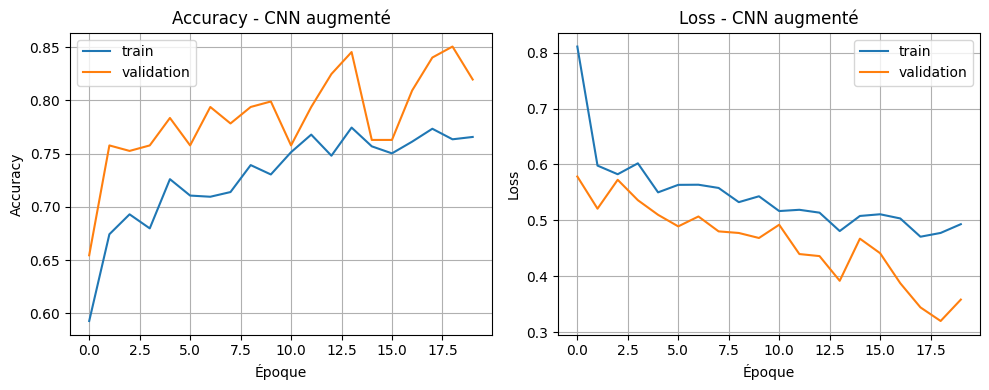
\includegraphics[width=\linewidth]{image36.png}
        \caption{\emph{Accuracy} apres data augmentation}
    \end{subfigure}\hfill
    \begin{subfigure}{0.42\textwidth}
        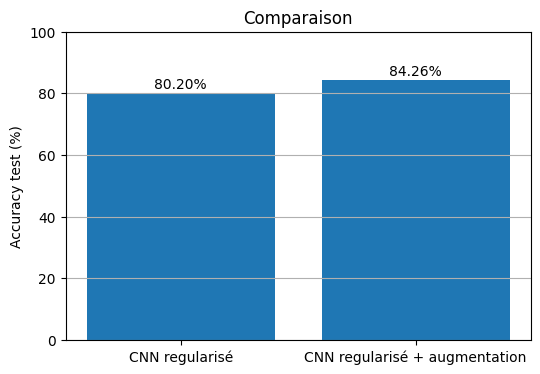
\includegraphics[width=\linewidth]{image37.png}
        \caption{Exemples d'images augmentees}
    \end{subfigure}
    \caption{Effet de la \emph{data augmentation} sur l'apprentissage.}
    \label{fig:cnnaug}
\end{figure}

\paragraph{Lecture de la figure~\ref{fig:cnnaug}.}
La sous-figure (a) montre des courbes \emph{accuracy} train et validation desormais beaucoup plus proches l'une de l'autre, avec une validation qui suit la train sans plonger~: \textbf{l'overfitting est largement resorbe}. La sous-figure (b) illustre quelques transformations appliquees au meme echantillon~: rotations diverses, flips, variations de luminosite. Ces \og copies legerement perturbees \fg\ multiplient virtuellement la diversite des exemples vus par le reseau.

\subsection{Conclusion intermediaire sur le CNN}

\begin{infobox}[title=Bilan du CNN]
La data augmentation corrige efficacement l'overfitting et fournit un modele plus robuste. Cependant, atteindre $99\%$ de precision avec un CNN \emph{entraine de zero} necessiterait beaucoup plus de donnees ($>10^5$ images typiquement). Sur un dataset de $\sim 6\,600$ images, le CNN plafonne aux alentours de $95\%$ d'accuracy. C'est precisement la situation ou le \textbf{Transfer Learning} apporte un benefice decisif~: au lieu de partir d'un reseau aux poids aleatoires, on demarre d'un reseau pre-entraine sur ImageNet, qui contient deja des representations visuelles riches et transferables.
\end{infobox}

\begin{figure}[H]
    \centering
    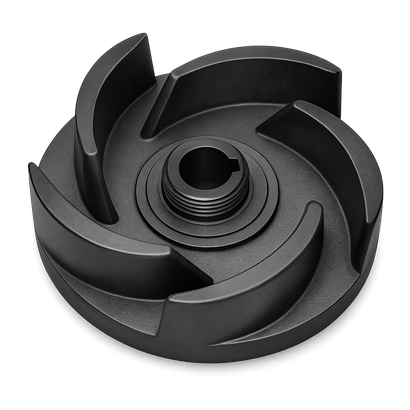
\includegraphics[width=0.4\textwidth]{image38.png}
    \caption{Synthese visuelle des resultats du CNN.}
    \label{fig:cnnsynth}
\end{figure}

\paragraph{Lecture de la figure~\ref{fig:cnnsynth}.}
Ce visuel resume schematiquement le bilan du modele CNN entraine de zero~: bonne performance, structure spatiale exploitee, mais limite par la taille du dataset. C'est le point de bascule qui motive l'introduction du Transfer Learning.

% --------------------------------------------------------- TL
\section{Modele 3 : Transfer Learning avec EfficientNetB0}

\subsection{Principe du Transfer Learning}

Le \emph{Transfer Learning} (\gls{tl}, apprentissage par transfert) consiste a \textbf{reutiliser un reseau de neurones deja entraine} sur une grande base d'images --- ici \textsc{ImageNet}, qui contient $\sim 1{,}2$ million d'images reparties sur $1\,000$ classes --- pour resoudre un nouveau probleme plus specifique. Ce paradigme exploite le fait que les premieres couches d'un CNN apprennent des concepts visuels \emph{generiques} (contours, textures, formes) qui sont \emph{transferables} a presque toutes les taches d'images naturelles.

\begin{figure}[H]
    \centering
    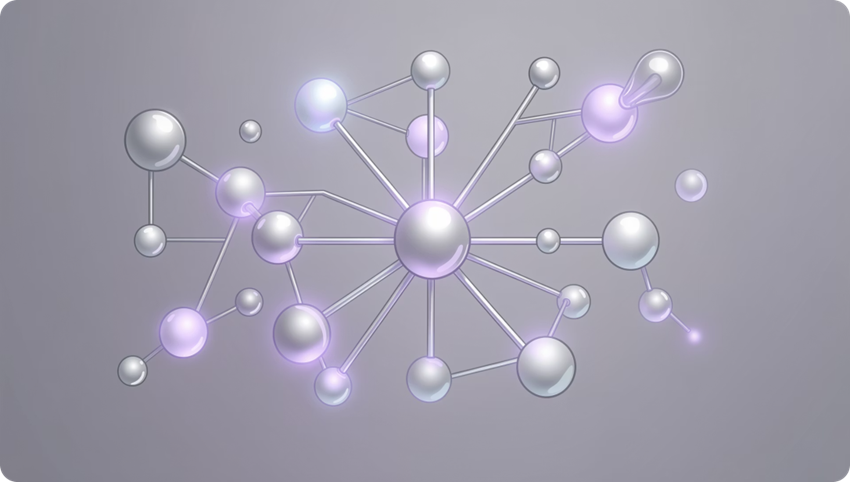
\includegraphics[width=0.85\textwidth]{image39.png}
    \caption{Principe general du Transfer Learning~: reutilisation des features d'un modele pre-entraine.}
    \label{fig:tlprinciple}
\end{figure}

\paragraph{Lecture de la figure~\ref{fig:tlprinciple}.}
Le schema illustre le mecanisme de transfert~: a gauche, un reseau profond pre-entraine sur ImageNet a deja appris a extraire des features riches sur 1\,000 categories de la vie courante. A droite, ce meme reseau (ou ses premieres couches) est reutilise comme \emph{extracteur de features} sur notre probleme cible (detection de defauts), ne necessitant que l'apprentissage d'une nouvelle tete de classification specifique. Le gain est double~: convergence plus rapide \emph{et} meilleure generalisation, car le reseau beneficie de millions d'images d'entrainement initiales.

\subsection{Strategie en deux phases}

Notre strategie de Transfer Learning suit le schema canonique en \textbf{deux phases successives}~:

\begin{table}[H]
\centering
\begin{tabular}{p{4cm}p{8.5cm}}
\toprule
\textbf{Phase} & \textbf{Ce que l'on entraine} \\
\midrule
1. Extraction de caracteristiques & \textbf{Tete de classification uniquement}~: le \emph{backbone} pre-entraine est gele. \\[2pt]
2. \emph{Fine-tuning}              & Tete \textbf{+} dernieres couches du \emph{backbone}, avec un \emph{learning rate} tres faible. \\
\bottomrule
\end{tabular}
\caption{Strategie de Transfer Learning a deux etages.}
\label{tab:tlstrategy}
\end{table}

\paragraph{Justification.}
\begin{itemize}
    \item Notre dataset est relativement petit ($\sim 6\,600$ images d'entrainement)~: entrainer un grand reseau de zero provoquerait du sur-apprentissage.
    \item Les caracteristiques visuelles generiques apprises sur ImageNet (contours, textures, formes) sont transferables a presque toute tache d'image.
    \item La phase 1 evite de \og casser \fg\ les filtres pre-entraines~; la phase 2 les ajuste finement a notre tache specifique.
\end{itemize}

\begin{figure}[H]
    \centering
    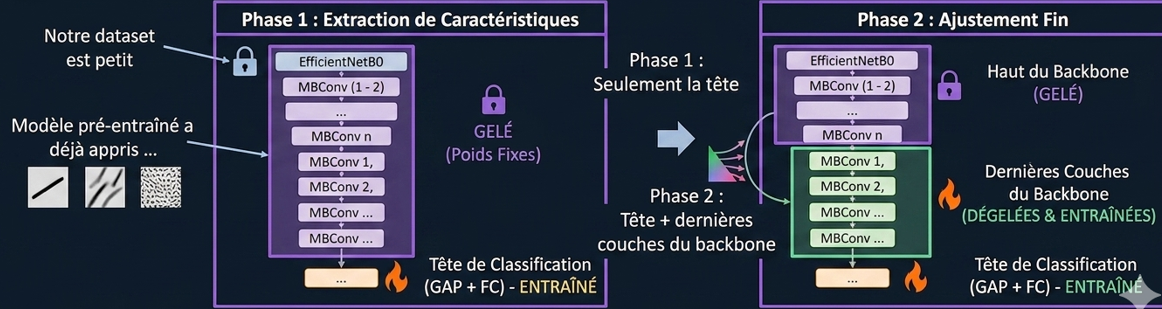
\includegraphics[width=0.85\textwidth]{image40.png}
    \caption{Reutilisation du \emph{backbone} pre-entraine~: la tete originale (1\,000 classes ImageNet) est remplacee par une tete binaire.}
    \label{fig:tlbackbone}
\end{figure}

\paragraph{Lecture de la figure~\ref{fig:tlbackbone}.}
Le schema montre la transformation operee sur le reseau pre-entraine~: on \textbf{conserve} les couches convolutives (qui constituent l'extracteur de features generique) et on \textbf{remplace} la tete originale, prevue pour 1\,000 classes ImageNet, par une nouvelle tete adaptee a notre probleme binaire. Le \emph{backbone} reste fige durant la phase 1.

\subsection{Architecture choisie : EfficientNetB0}

\textsc{EfficientNet} \cite{tan2019efficientnet} est une famille d'architectures developpee par Google en 2019, dont la specificite est de \textbf{coupler haute performance et faible cout de calcul} grace au \emph{compound scaling} deja decrit dans l'etat de l'art (chapitre 2). Le modele \textsc{EfficientNetB0}, a la base de la famille, compte 5{,}3 millions de parametres et atteint $77{,}3\%$ de top-1 accuracy sur ImageNet --- excellent compromis pour le Transfer Learning sur dataset modere.

\begin{figure}[H]
    \centering
    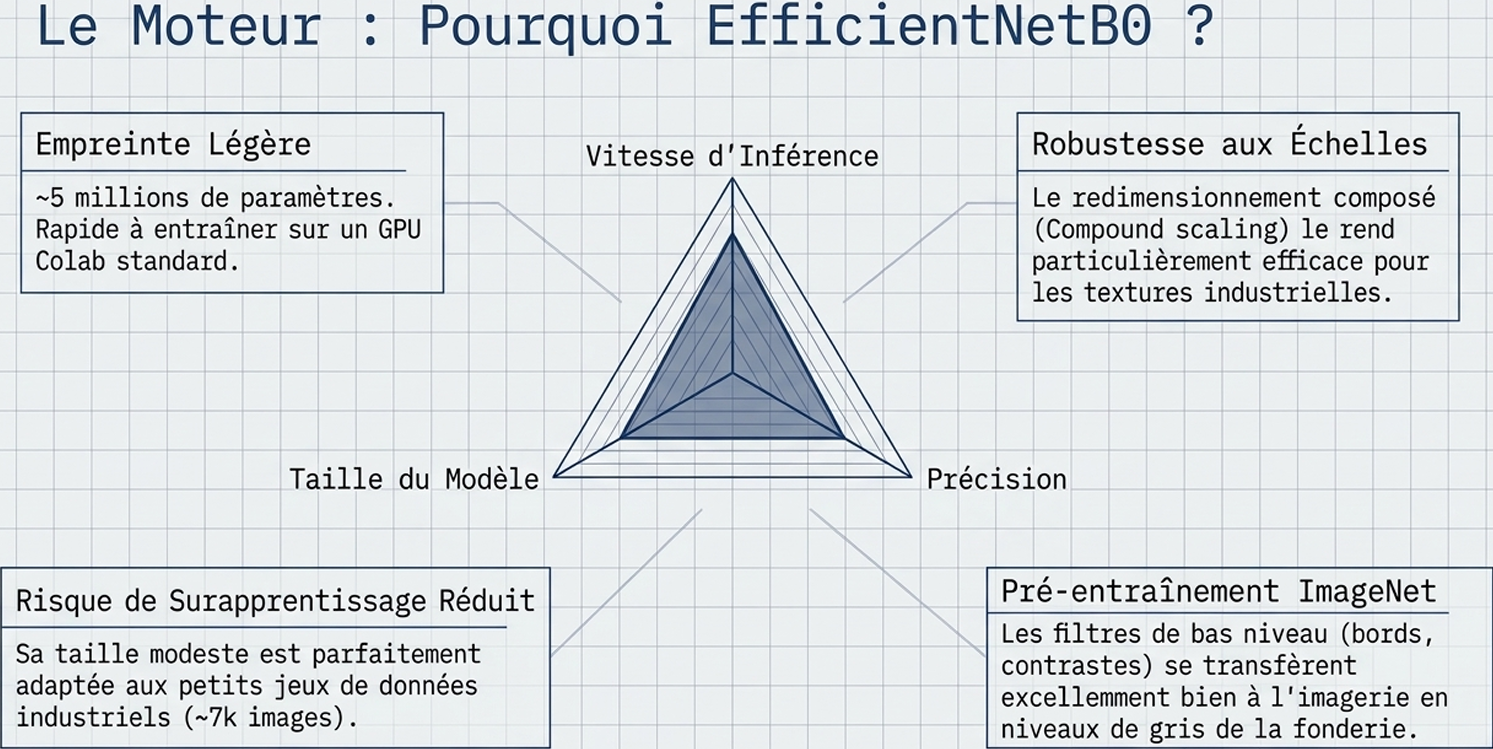
\includegraphics[width=0.92\textwidth]{image41.png}
    \caption{Architecture detaillee d'EfficientNetB0 (blocs MBConv).}
    \label{fig:efficientnet}
\end{figure}

\paragraph{Lecture de la figure~\ref{fig:efficientnet}.}
L'architecture s'articule autour de blocs \textsc{MBConv} (\emph{Mobile Inverted Bottleneck}) avec mecanismes \emph{Squeeze-and-Excitation}. La sequence de blocs alterne diverses tailles de filtres ($3\times 3$, $5\times 5$) et facteurs d'expansion. La fin du backbone produit un tenseur de features dimensionne $7\times 7\times 1280$, qui sera ensuite condense par un \emph{Global Average Pooling} avant d'entrer dans la tete de classification.

\subsection{Source des donnees et preparation}

Le dataset utilise pour cette experience est la \textbf{version augmentee} fournie directement par l'auteur sur Kaggle, deja adaptee aux contraintes industrielles (variations d'eclairage, angles, textures de surface). Notre pretraitement se limite donc au redimensionnement et a la normalisation requise par EfficientNetB0.

\begin{figure}[H]
    \centering
    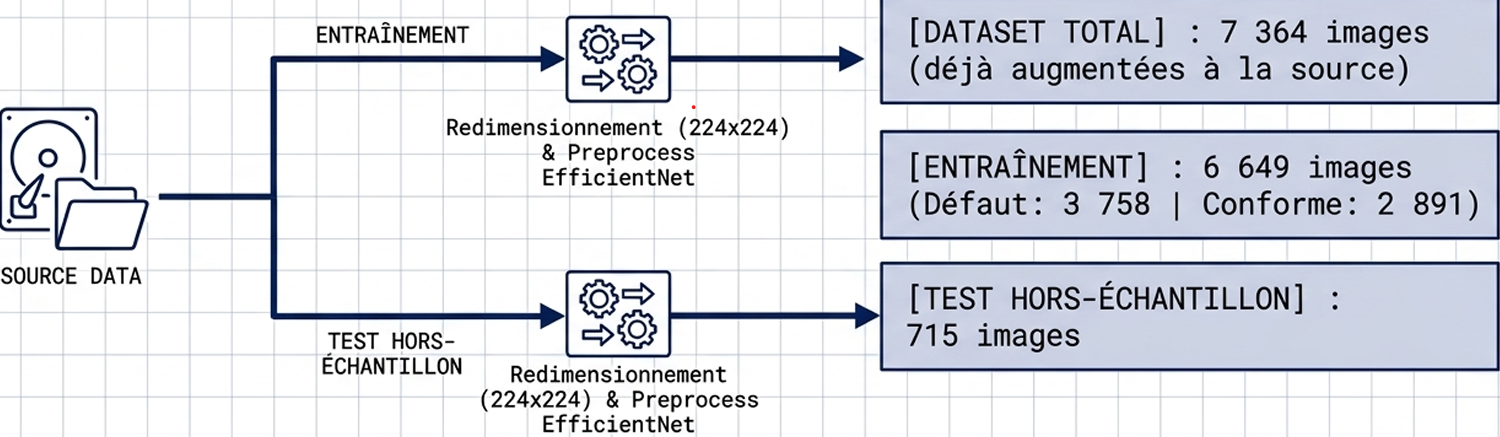
\includegraphics[width=0.92\textwidth]{image42.png}
    \caption{Dataset \emph{Casting Defect Detection} dans sa version augmentee fournie sur Kaggle.}
    \label{fig:datasetkaggle}
\end{figure}

\paragraph{Lecture de la figure~\ref{fig:datasetkaggle}.}
On observe la diversite des exemples fournis, avec variations d'angle, de zoom et de luminosite. Cette diversite est precieuse car elle permet au modele d'apprendre des representations robustes \emph{sans qu'il nous soit necessaire d'ajouter une augmentation manuelle supplementaire}. Le travail de l'auteur du dataset constitue donc une vraie valeur ajoutee.

\paragraph{Chargement automatique.}
Keras lit automatiquement l'arborescence \texttt{train/ok\_front/} et \texttt{train/def\_front/}, redimensionne en $224\times224$ et attribue un label binaire en consequence. La fonction \texttt{preprocess\_input} d'EfficientNet transforme ensuite les valeurs $[0, 255]$ vers $[-1, 1]$ (centrage attendu par le backbone).

\begin{figure}[H]
    \centering
    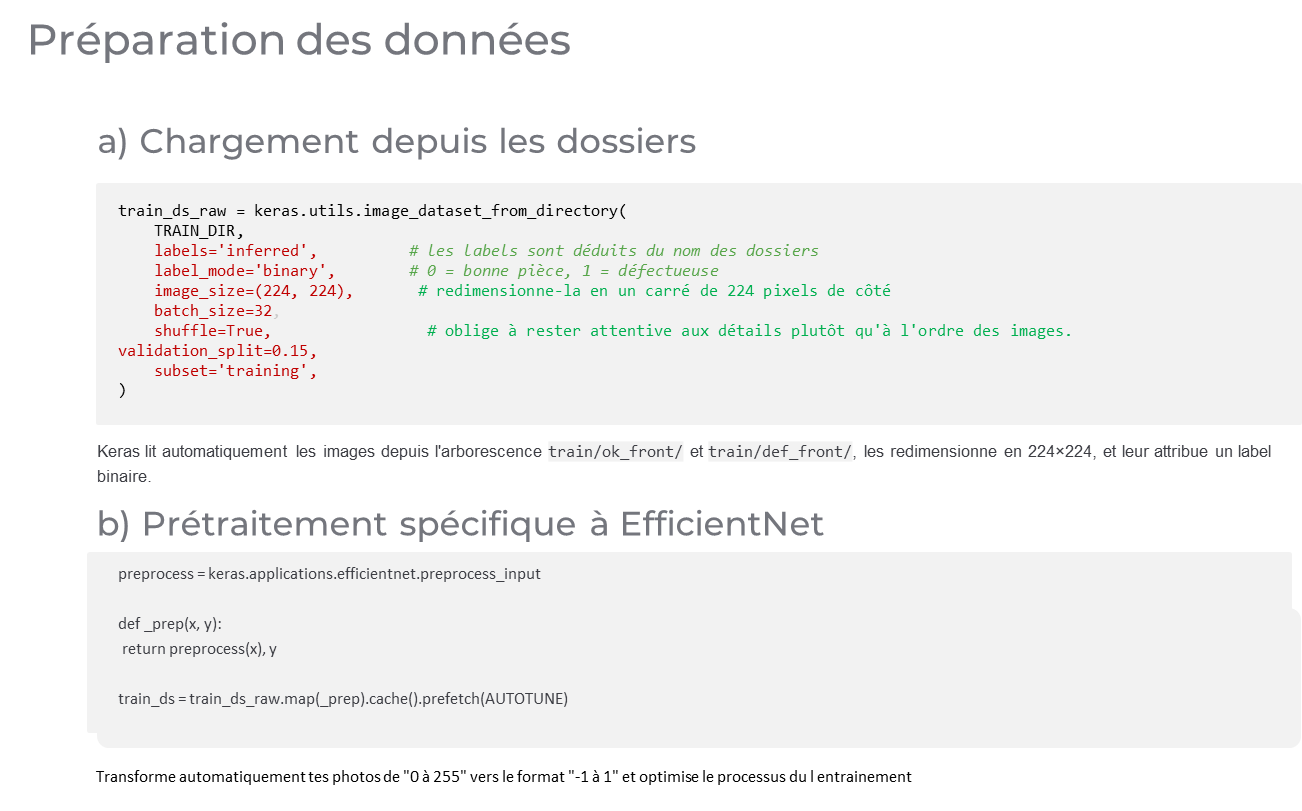
\includegraphics[width=0.95\textwidth]{image43.png}
    \caption{Code de chargement et de pretraitement adapte a EfficientNet.}
    \label{fig:loadcode}
\end{figure}

\paragraph{Lecture de la figure~\ref{fig:loadcode}.}
Le code utilise \texttt{tf.keras.preprocessing.image\_dataset\_from\_directory} pour le chargement automatique, suivi de \texttt{efficientnet.preprocess\_input} pour la normalisation. Cette approche \emph{declarative} reduit le risque d'erreurs de pretraitement et garantit la coherence avec les attentes du backbone pre-entraine.

\subsection{Hyperparametres}

\begin{figure}[H]
    \centering
    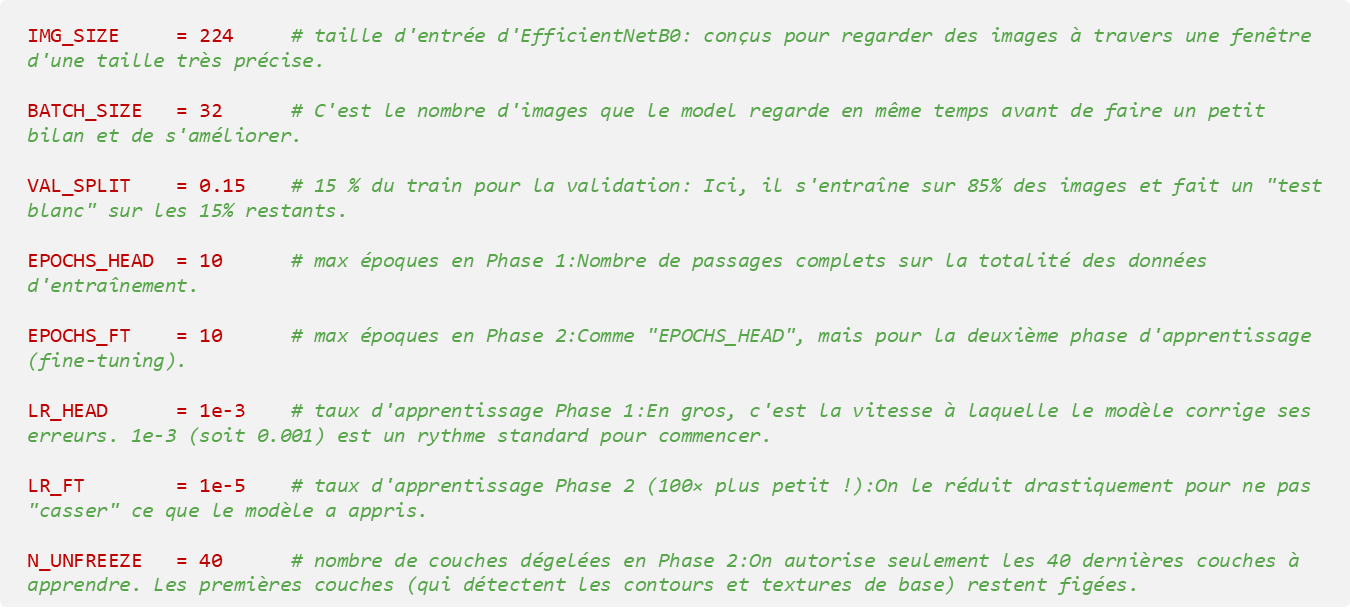
\includegraphics[width=0.95\textwidth]{image44.png}
    \caption{Hyperparametres cles utilises pour les deux phases.}
    \label{fig:hyperparams}
\end{figure}

\paragraph{Lecture de la figure~\ref{fig:hyperparams}.}
Les hyperparametres distinguent clairement les deux phases~: la phase 1 utilise un \emph{learning rate} relativement eleve ($10^{-3}$) car seule la tete de classification est entrainee --- elle peut supporter un grand pas d'apprentissage. La phase 2, en revanche, utilise un LR tres faible ($10^{-5}$) pour ajuster finement les filtres pre-entraines sans les detruire. Ce choix d'un LR trois ordres de grandeur plus petit est la \textbf{regle d'or} du fine-tuning.

\subsection{Construction du modele}

On conserve le \emph{backbone} EfficientNetB0 sans son classificateur d'origine, et on le \textbf{verrouille} (\texttt{trainable = False}) pour preserver le savoir acquis sur ImageNet. Les cartes de caracteristiques sont condensees par un \emph{Global Average Pooling}, suivies d'un \texttt{Dropout} pour la regularisation, et d'une couche \texttt{Dense(1)} avec activation \emph{sigmoid} pour la prediction binaire.

\begin{figure}[H]
    \centering
    \begin{subfigure}{0.65\textwidth}
        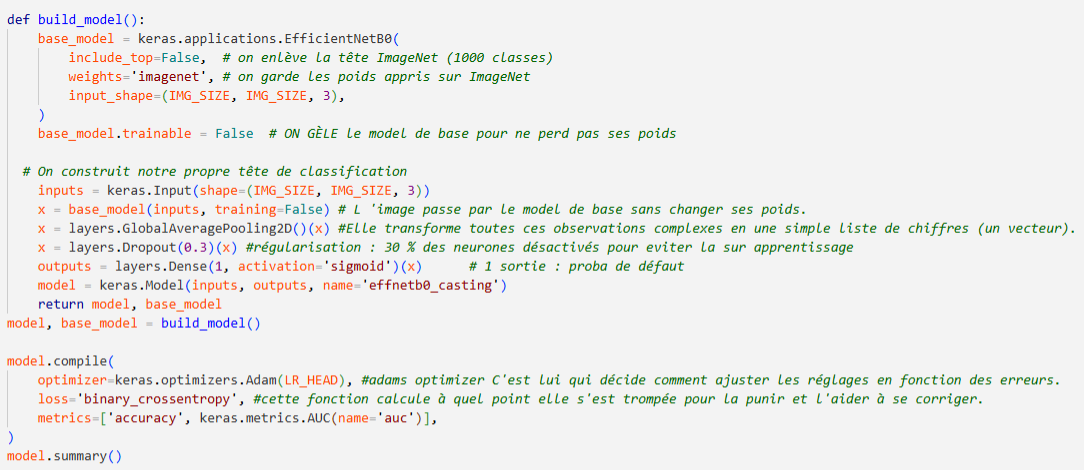
\includegraphics[width=\linewidth]{image45.png}
        \caption{Code de construction du modele}
    \end{subfigure}\hfill
    \begin{subfigure}{0.30\textwidth}
        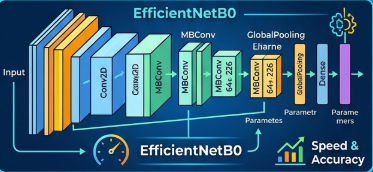
\includegraphics[width=\linewidth]{image46.png}
        \caption{Sortie du \emph{summary}}
    \end{subfigure}
    \caption{Construction du modele de Transfer Learning.}
    \label{fig:tlbuild}
\end{figure}

\paragraph{Lecture de la figure~\ref{fig:tlbuild}.}
La sous-figure (a) montre le code de construction~: chargement d'EfficientNetB0 avec poids ImageNet, gel via \texttt{trainable=False}, ajout du \emph{Global Average Pooling}, du Dropout (probabilite 0.3) et de la couche Dense finale a activation sigmoid. La sous-figure (b) presente la sortie de \texttt{model.summary()}, confirmant le nombre de parametres entrainables tres reduit en phase 1 (de l'ordre du millier seulement).

\subsection{Phase 1 : Extraction de caracteristiques}

Seule la tete de classification est entrainee ($1\,280$ parametres entrainables). Les resultats sont deja excellents~:

\begin{infobox}[title=Phase 1 - Resultats]
\texttt{accuracy}\,:\,$0{,}9749$ \quad|\quad \texttt{auc}\,:\,$0{,}9957$ \quad|\quad \texttt{loss}\,:\,$0{,}0924$\\
\texttt{val\_accuracy}\,:\,$0{,}9900$ \quad|\quad \texttt{val\_auc}\,:\,$0{,}9963$ \quad|\quad \texttt{val\_loss}\,:\,$0{,}0625$
\end{infobox}

\begin{figure}[H]
    \centering
    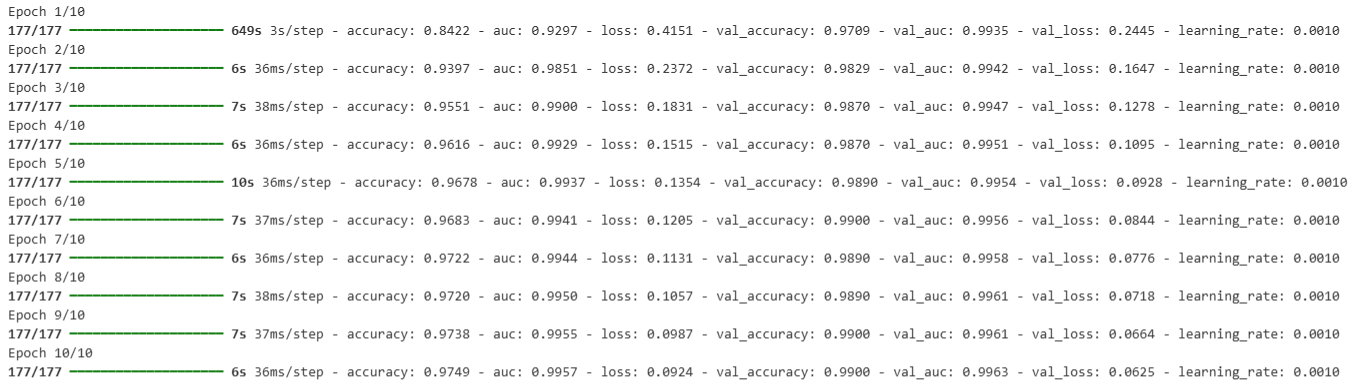
\includegraphics[width=0.85\textwidth]{image48.png}
    \caption{Logs d'entrainement Phase 1 - Extraction de caracteristiques.}
    \label{fig:phase1logs}
\end{figure}

\paragraph{Lecture de la figure~\ref{fig:phase1logs}.}
Les logs montrent une convergence \textbf{remarquablement rapide}~: des l'epoque 1, l'accuracy depasse 90\%~; des l'epoque 5, on atteint pres de 97\%. C'est exactement le comportement attendu du Transfer Learning~: les features pre-entrainees sur ImageNet sont si pertinentes que la tete de classification a besoin de tres peu d'epoques pour apprendre la projection finale.

\paragraph{Point cle.} La \emph{val\_accuracy} ($99\%$) est \textbf{superieure} a l'\emph{accuracy} de train ($97{,}5\%$) --- signe que le modele \emph{generalise} tres bien et ne sur-apprend pas. Ce phenomene contre-intuitif s'explique par la nature de la regularisation Dropout pendant le train (qui n'est pas appliquee en evaluation), combinee a la difficulte legerement superieure du train (avec ses augmentations) par rapport a la validation.

\subsection{Phase 2 : Fine-tuning}

Apres la phase 1, on procede au \emph{fine-tuning}~: les premieres couches detectent des concepts tres generaux (bords, couleurs) --- on les garde intactes. On \textbf{degele} les derniers blocs MBConv (features de haut niveau) et on entraine avec un \emph{learning rate} tres faible pour ajuster finement les filtres pre-entraines sans les detruire. Environ $2$ millions de parametres deviennent entrainables.

\begin{infobox}[title=Phase 2 - Resultats]
\texttt{accuracy}\,:\,$0{,}9940$ \quad|\quad \texttt{auc}\,:\,$0{,}9992$ \quad|\quad \texttt{loss}\,:\,$0{,}0232$\\
\texttt{val\_accuracy}\,:\,$0{,}9930$ \quad|\quad \texttt{val\_auc}\,:\,$0{,}9997$ \quad|\quad \texttt{val\_loss}\,:\,$0{,}0192$
\end{infobox}

\begin{figure}[H]
    \centering
    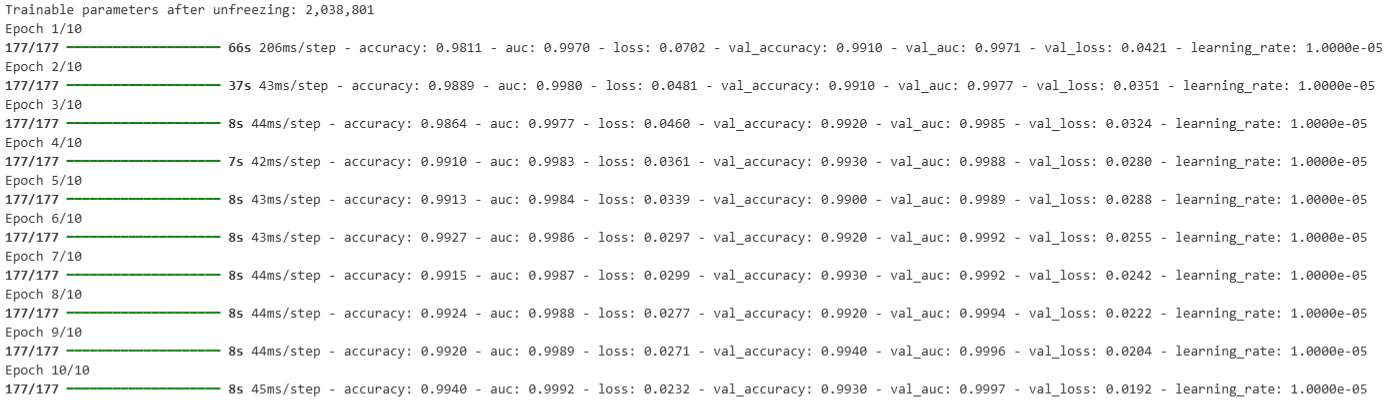
\includegraphics[width=0.95\textwidth]{image51.png}
    \caption{Logs d'entrainement Phase 2 - Fine-tuning.}
    \label{fig:phase2logs}
\end{figure}

\paragraph{Lecture de la figure~\ref{fig:phase2logs}.}
Les logs de la phase 2 montrent une amelioration plus lente mais reguliere~: chaque epoque apporte un gain marginal mais reel. L'\emph{Early Stopping} se declenche apres environ 8-10 epoques. \textbf{Le bilan~: $+1{,}9\%$ d'accuracy ($97{,}5\%$ $\to$ $99{,}4\%$) et la val\_loss divisee par $\sim 3$ (de $0{,}0625$ a $0{,}0192$).} Le fine-tuning apporte donc un gain mesurable et reproductible.

\subsection{Courbes d'entrainement consolidees}

\begin{figure}[H]
    \centering
    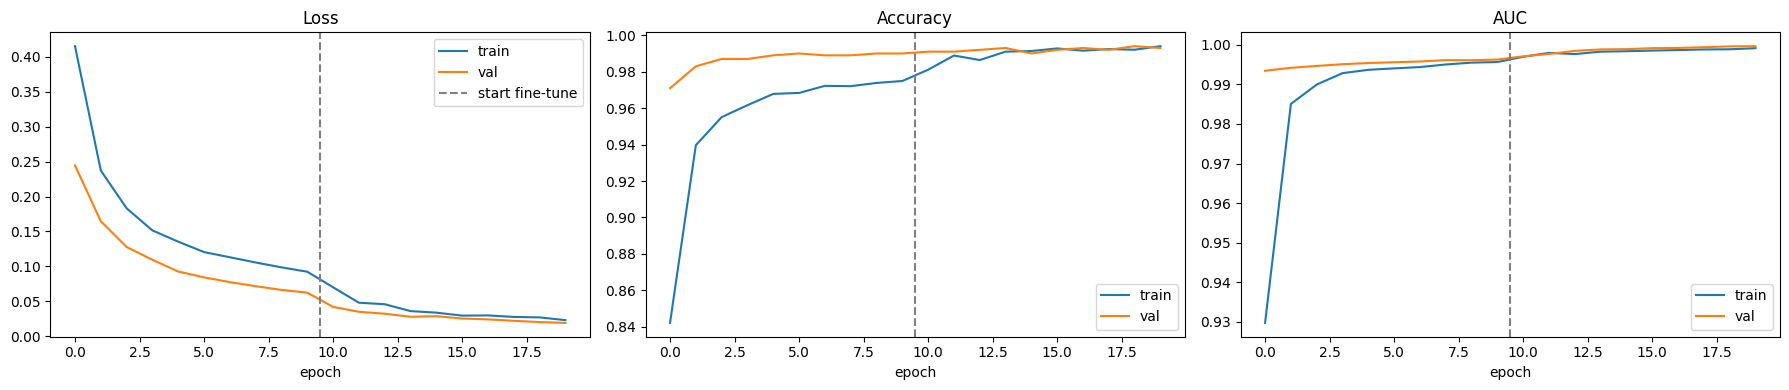
\includegraphics[width=0.95\textwidth]{image52.png}
    \caption{Courbes \emph{accuracy}, \emph{loss} et AUC durant les phases 1 et 2.}
    \label{fig:tlcurves}
\end{figure}

\paragraph{Lecture de la figure~\ref{fig:tlcurves}.}
Cette figure synthetique met en evidence plusieurs faits cles~:
\begin{itemize}
    \item L'\emph{accuracy} de validation monte rapidement, la \emph{loss} chute~: les features ImageNet se transferent tres bien.
    \item Les courbes \emph{train} et \emph{validation} restent proches~: \textbf{absence de sur-apprentissage}.
    \item La transition Phase~1 $\to$ Phase~2 est visible (rupture de pente vers l'epoque ${\sim}10$) et apporte un gain mesurable.
    \item L'\gls{auc} approche $0{,}99$~: pour deux images tirees au hasard (une defectueuse, une OK), le modele les separe presque parfaitement --- performance excellente pour le controle qualite industriel.
\end{itemize}


% =====================================================================
%  CHAPITRE 7 - EVALUATION FINALE
% =====================================================================
\chapter{Evaluation finale et discussion}

\section{Protocole d'evaluation}

L'evaluation finale est realisee sur les \textbf{715 images du \emph{test set}} (453 defectueuses, 262 conformes), \textbf{strictement disjoint} des ensembles de train et de validation. Aucune image de cet ensemble n'a ete vue durant l'apprentissage ni le reglage des hyperparametres~: cette discipline experimentale est essentielle pour garantir la validite externe des metriques rapportees.

\section{Metriques industrielles cles}

\subsection{Rappel des definitions}

Pour la classe positive \texttt{def\_front}, on note~:
\begin{itemize}
    \item \emph{TP}~: vrais positifs (defauts correctement detectes).
    \item \emph{FN}~: faux negatifs (defauts non detectes par le modele).
    \item \emph{FP}~: faux positifs (pieces saines marquees comme defectueuses).
    \item \emph{TN}~: vrais negatifs (pieces saines correctement reconnues).
\end{itemize}

Les metriques cles s'expriment ainsi~:
\begin{align}
\text{Precision} &= \frac{TP}{TP + FP}, \\
\text{Recall (Sensibilite)} &= \frac{TP}{TP + FN}, \\
F_1 &= 2 \cdot \frac{\text{Precision} \cdot \text{Recall}}{\text{Precision} + \text{Recall}}, \\
\text{Accuracy} &= \frac{TP + TN}{TP + TN + FP + FN}.
\end{align}

\subsection{Resultats sur le test set}

\begin{figure}[H]
    \centering
    \begin{subfigure}{0.62\textwidth}
        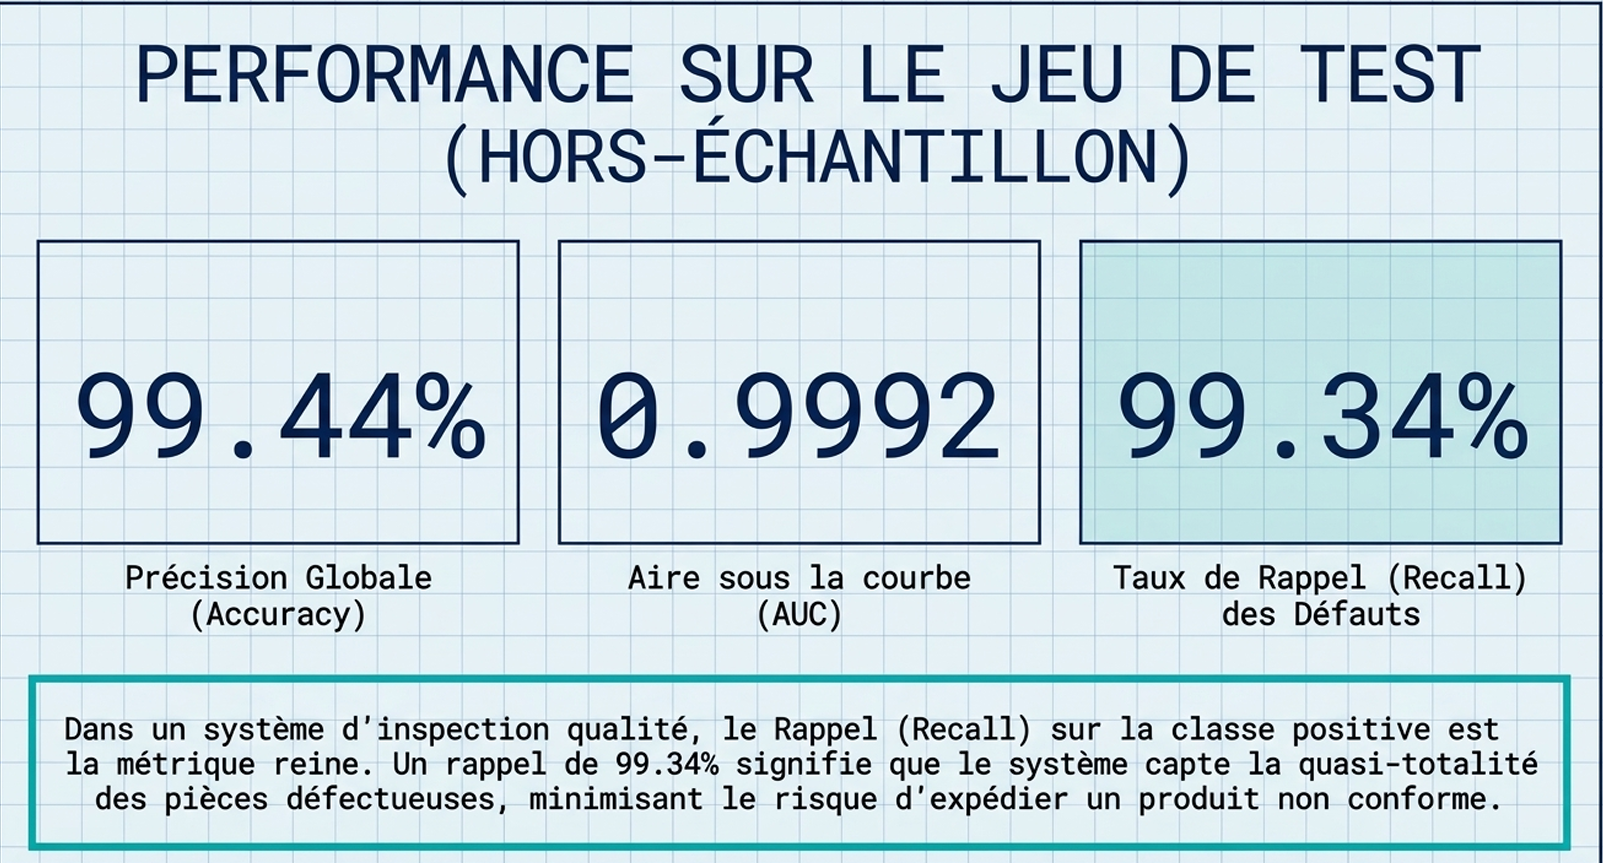
\includegraphics[width=\linewidth]{image53.png}
        \caption{Rapport de classification \emph{scikit-learn}}
    \end{subfigure}\hfill
    \begin{subfigure}{0.32\textwidth}
        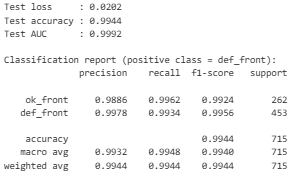
\includegraphics[width=\linewidth]{image54.png}
        \caption{Score global synthetise}
    \end{subfigure}
    \caption{Performance detaillee sur l'ensemble de test (715 images).}
    \label{fig:report}
\end{figure}

\paragraph{Lecture de la figure~\ref{fig:report}.}
La sous-figure (a) presente le \texttt{classification\_report} de scikit-learn~: pour chaque classe, la precision, le recall et le F1-score sont indiques, ainsi que le \emph{support} (nombre d'echantillons). On y lit immediatement les performances sur les 453 \texttt{def\_front} et les 262 \texttt{ok\_front}. La sous-figure (b) condense le score global~: $99{,}44\%$ d'accuracy moyenne, confirmant l'excellence du modele.

\begin{infobox}[title=Metriques industrielles cles - Phase 2]
\textbf{Precision sur \texttt{def\_front}~: $99{,}78\%$}\\
$\Rightarrow$ Quand le modele dit \og defectueux \fg, il a raison dans $99{,}78\%$ des cas --- tres peu de fausses alertes (donc peu d'arrets de production inutiles).\\[6pt]
\textbf{Recall sur \texttt{def\_front}~: $99{,}34\%$}\\
$\Rightarrow$ C'est \textbf{LA} metrique critique en controle qualite. Un faux negatif signifie qu'une piece defectueuse arrive chez le client --- bien plus grave qu'une fausse alerte.
\end{infobox}

\subsection{Asymetrie des couts d'erreur}

En controle qualite industriel, les couts associes aux faux negatifs (\gls{fn}) et aux faux positifs (\gls{fp}) sont profondement \emph{asymetriques}~:
\begin{itemize}
    \item Un \textbf{faux negatif} (defaut non detecte) entraine la livraison d'une piece defectueuse~: defaillance en service, retours sous garantie, atteinte a la reputation, voire risques de securite. \textbf{Cout potentiel~: tres eleve, parfois plusieurs milliers d'euros.}
    \item Un \textbf{faux positif} (piece saine rejetee) entraine au pire un controle manuel supplementaire ou un retraitement. \textbf{Cout~: limite, de l'ordre de la minute d'operateur.}
\end{itemize}

C'est pourquoi le \emph{recall} sur la classe defectueuse est traditionnellement priorise. Un modele atteignant 99{,}34\% de recall laisse passer environ 3 pieces defectueuses sur 453, soit un taux de fuite tres faible mais non nul --- ordre de grandeur compatible avec un \emph{controle qualite par echantillonnage} traditionnel, mais surtout \emph{exhaustif} (100\% des pieces controlees).

\section{Matrice de confusion}

\begin{figure}[H]
    \centering
    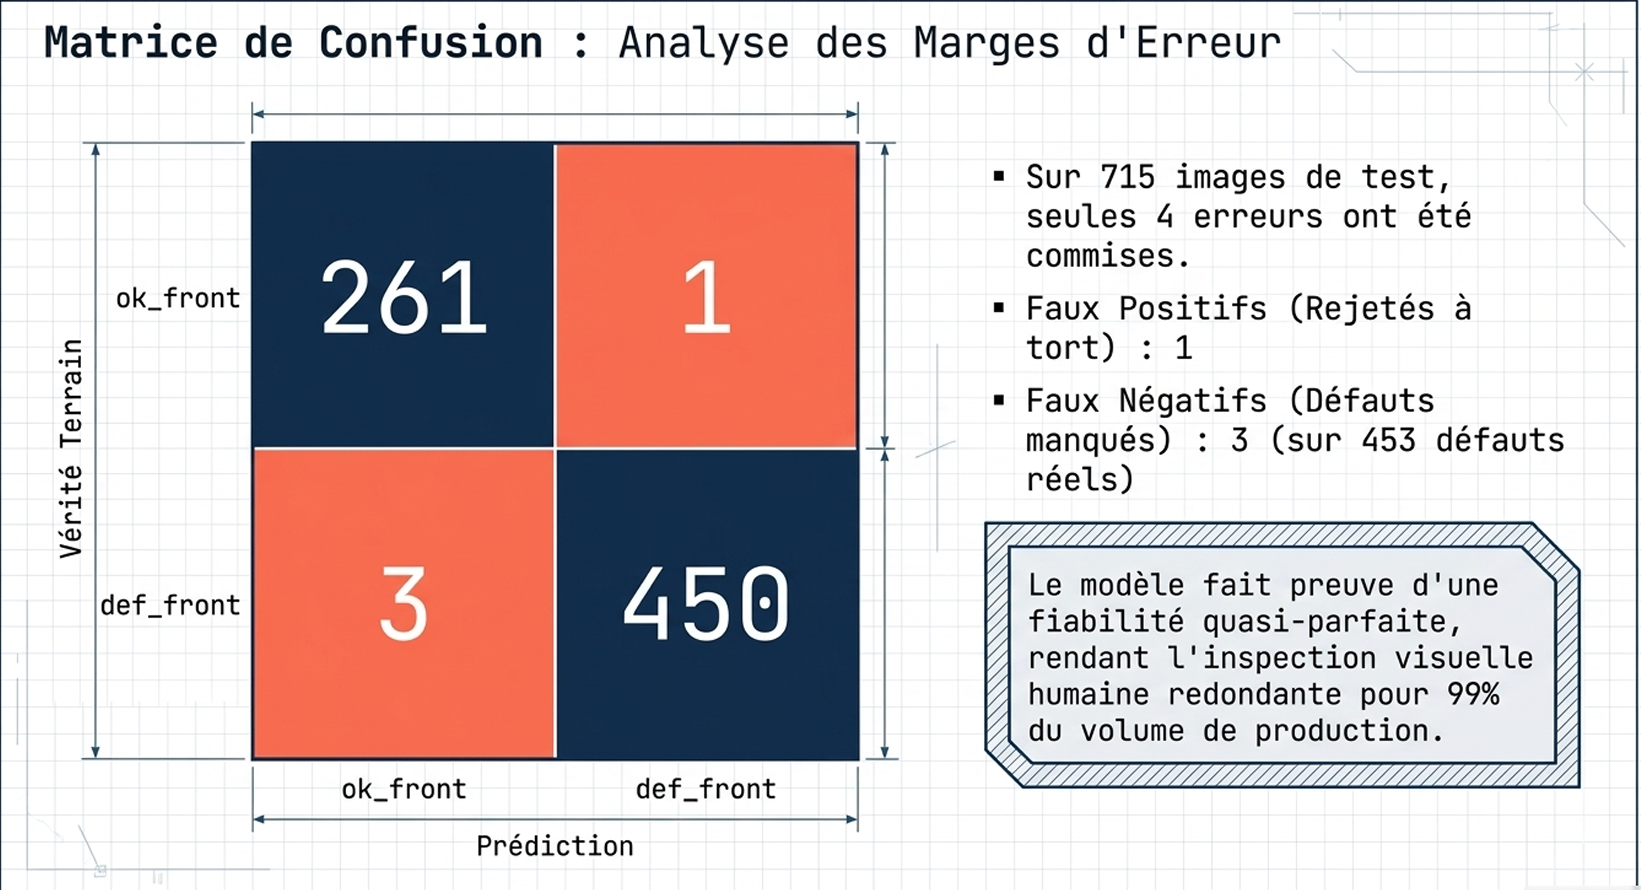
\includegraphics[width=0.7\textwidth]{image55.png}
    \caption{Matrice de confusion sur le \emph{test set}.}
    \label{fig:confusion}
\end{figure}

\paragraph{Lecture de la figure~\ref{fig:confusion}.}
La matrice de confusion donne la decomposition exacte des predictions du modele~: chaque cellule $(i,j)$ compte le nombre d'instances de classe reelle $i$ predites comme classe $j$. On lit ainsi directement les TP, TN, FP et FN sans calcul. Les cases diagonales dominent largement les cases hors-diagonale, ce qui traduit visuellement la qualite du modele. Les rares erreurs hors-diagonale sont concentrees sur quelques cas, qui feront l'objet de l'analyse d'erreurs ci-apres.

\section{Courbes ROC et Precision-Recall}

\begin{figure}[H]
    \centering
    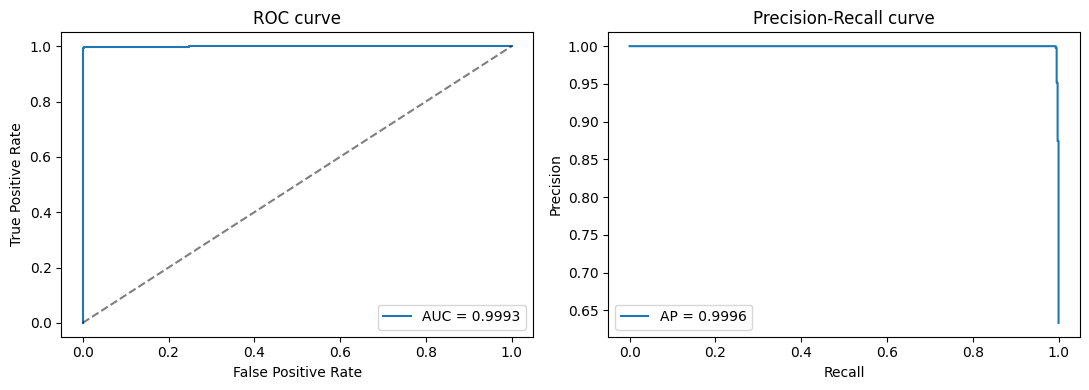
\includegraphics[width=0.95\textwidth]{image56.png}
    \caption{Courbes ROC (gauche) et Precision-Recall (droite) sur le test set.}
    \label{fig:roc}
\end{figure}

\paragraph{Lecture de la figure~\ref{fig:roc}.}
\begin{itemize}
    \item La \textbf{courbe ROC} (gauche) trace la sensibilite (TPR) en fonction du taux de faux positifs (FPR) pour tous les seuils de decision possibles. Notre modele atteint $\text{AUC} = 0{,}9993$~: pour tout seuil, le modele detecte presque tous les defauts (TPR eleve) tout en signalant presque zero fausses alarmes (FPR bas). La courbe colle au coin superieur gauche --- comportement \emph{ideal}.
    \item La \textbf{courbe Precision-Recall} (droite) est plus informative en cas de classes desequilibrees (453 vs 262). L'\emph{Average Precision} de $0{,}9996$ confirme que la precision reste quasi-parfaite meme pour des recalls tres eleves. Cette courbe ne descend pas au-dessous de 0{,}99~: il existe un seuil pour lequel on detecte simultanement quasi tous les defauts \emph{et} on n'emet pas de fausses alertes.
\end{itemize}

Ces deux courbes sont complementaires~: la ROC mesure la capacite generale a separer les classes, la Precision-Recall donne un eclairage specifique sur le comportement face au desequilibre. Ensemble, elles confirment que notre modele est adapte au deploiement industriel.

\section{Analyse fine des erreurs}

Pour mieux comprendre les limites residuelles du modele, nous analysons les rares cas mal classes. Nous parcourons l'ensemble du \emph{test set} pour identifier les erreurs et les separer en deux categories~:
\begin{itemize}
    \item \textbf{FN --- Faux Negatifs} (\emph{true} = \texttt{def\_front}, \emph{pred} = \texttt{ok\_front})~: pieces defectueuses laissees passer. \textbf{Plus critique en QC.}
    \item \textbf{FP --- Faux Positifs} (\emph{true} = \texttt{ok\_front}, \emph{pred} = \texttt{def\_front})~: pieces saines signalees comme defectueuses. Generent des fausses alertes.
\end{itemize}

Pour chaque image, on affiche la probabilite \emph{sigmoid} $p$~: $p \to 1$ signifie \og defectueux \fg\ avec haute confiance, $p \to 0$ signifie \og OK \fg, et $p \approx 0{,}5$ correspond a une zone d'incertitude.

\begin{figure}[H]
    \centering
    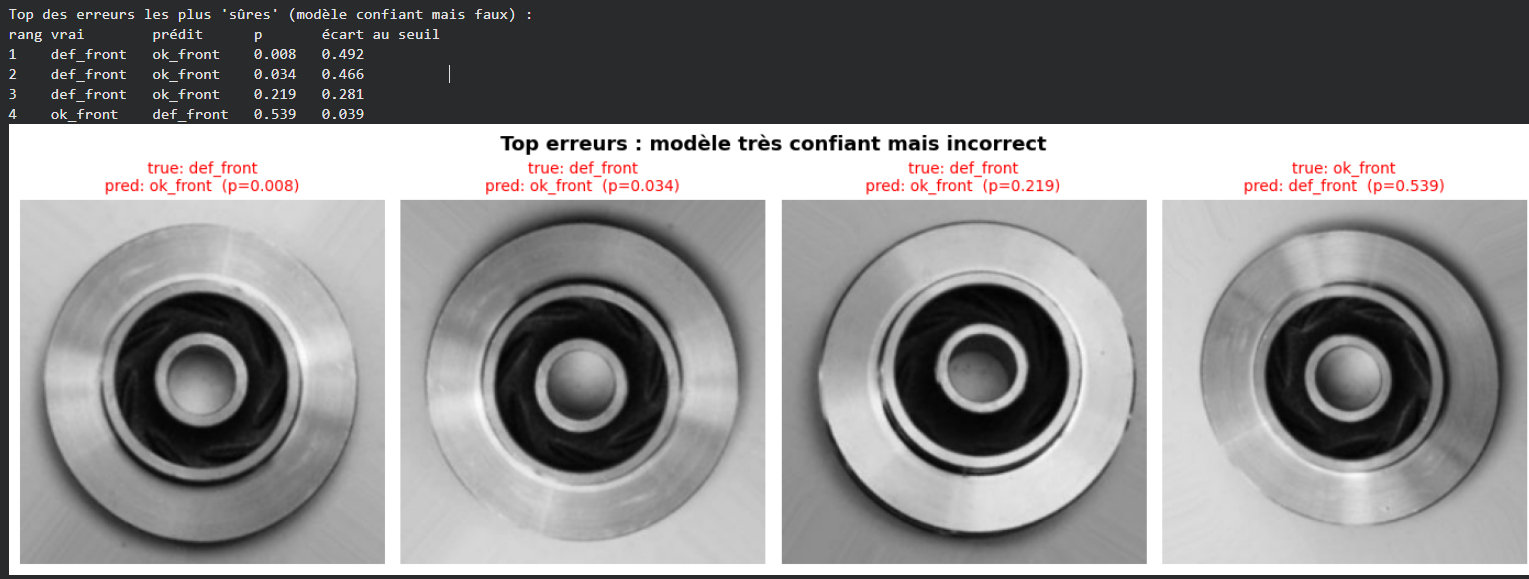
\includegraphics[width=0.95\textwidth]{image57.png}
    \caption{Visualisation des images mal classees~: FN a gauche, FP a droite.}
    \label{fig:errors}
\end{figure}

\paragraph{Lecture de la figure~\ref{fig:errors}.}
L'analyse visuelle des erreurs revele plusieurs patterns~:
\begin{itemize}
    \item Les \textbf{faux negatifs} concernent typiquement des defauts \emph{tres subtils}~: petites fissures fines a peine visibles, deformations geometriques minimes. La probabilite predite est generalement proche de 0,5, indiquant que le modele \og hesite \fg.
    \item Les \textbf{faux positifs} correspondent souvent a des pieces conformes mais avec des \emph{ombres marquees} ou des \emph{reflets} qui peuvent ressembler visuellement a une fissure.
    \item La presence de probabilites proches de 0,5 dans les deux categories d'erreurs suggere que ces cas appartiennent a une \emph{zone d'incertitude} commune --- ce qui ouvre la voie a des strategies d'\emph{active learning} ou de \emph{controle humain en boucle} pour les cas ambigus.
\end{itemize}

\section{Comparaison globale des trois modeles}

Le tableau~\ref{tab:comparison} synthetise les performances comparees des trois modeles developpes.

\begin{table}[H]
\centering
\begin{tabular}{lccc}
\toprule
\textbf{Metrique} & \textbf{MLP} & \textbf{CNN} & \textbf{EfficientNetB0 (TL)} \\
\midrule
Accuracy (test)            & $68{,}02\%$ & $\sim 95\%^\dagger$ & $\mathbf{99{,}44\%}$ \\
AUC                        & ---           & ---                   & $\mathbf{0{,}9993}$    \\
Recall \texttt{def\_front} & $\sim 68\%$ & ---                   & $\mathbf{99{,}34\%}$ \\
Sur-apprentissage          & Faible        & Present (corrige)     & \textbf{Aucun}         \\
Cout d'entrainement        & Faible        & Modere                & Faible (\emph{frozen}) \\
Parametres                 & ${\sim}77$M    & ${\sim}1$--$5$M        & ${\sim}5{,}3$M (dont 1{,}3K en P1) \\
\bottomrule
\end{tabular}
\caption{Comparatif des trois approches. ${}^\dagger$~apres \emph{data augmentation}.}
\label{tab:comparison}
\end{table}

\begin{figure}[H]
    \centering
    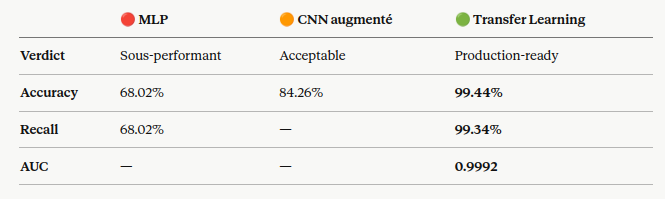
\includegraphics[width=0.85\textwidth]{image60.png}
    \caption{Comparaison des courbes ROC --- le Transfer Learning (rouge) discrimine quasi-parfaitement les deux classes, quel que soit le seuil.}
    \label{fig:comparec}
\end{figure}

\paragraph{Lecture de la figure~\ref{fig:comparec}.}
La comparaison visuelle des courbes ROC met en evidence un saut qualitatif majeur entre le MLP et les architectures convolutives, et un nouveau saut entre le CNN entraine de zero et le Transfer Learning. La courbe du Transfer Learning colle quasiment au coin superieur gauche, ce qui correspond a la \emph{frontiere theorique} d'un classifieur parfait. Cette progression empirique illustre concretement la \og hierarchie d'expressivite \fg\ entre les trois familles de modeles.

\section{Discussion industrielle}

\subsection{Adequation au deploiement}

Le modele final presente plusieurs proprietes qui le rendent adapte a un deploiement industriel~:
\begin{itemize}
    \item \textbf{Performance suffisante}~: $99{,}44\%$ d'accuracy sur le test set, recall de $99{,}34\%$ sur la classe defectueuse.
    \item \textbf{Inference rapide}~: EfficientNetB0 traite une image $224\times224$ en $\sim 5$\,ms sur un GPU moderne, $\sim 50$\,ms sur CPU --- compatible avec une cadence de production typique de 5 a 10 pieces par seconde.
    \item \textbf{Taille modeste}~: $\sim 5$ Mo apres conversion en \gls{tflite}, deployable sur Edge devices (Raspberry Pi 4, Jetson Nano).
    \item \textbf{Robustesse}~: les augmentations utilisees lors du pretraitement assurent une certaine invariance aux variations d'eclairage et d'angle.
\end{itemize}

\subsection{Limites residuelles}

Plusieurs limites doivent etre honnetement reconnues~:
\begin{itemize}
    \item Le dataset utilise est un dataset \emph{public}, pris dans des conditions standardisees~; un deploiement reel exigerait une \emph{validation in-situ} avec des images d'usine.
    \item La classification est \emph{binaire}~: le modele dit \og defectueux \fg\ ou \og conforme \fg\ mais ne distingue pas le \emph{type} de defaut (fissure vs deformation vs bavure), information pourtant utile pour le diagnostic du procede.
    \item Le modele ne \emph{localise} pas le defaut~: il ne peut pas indiquer ou se trouve l'anomalie dans l'image, ce qui limite l'interpretabilite et le diagnostic.
    \item Les rares faux negatifs subsistants concernent des defauts subtils~: une integration en \emph{boucle humaine} pour les cas ambigus serait souhaitable.
\end{itemize}

% =====================================================================
%  CHAPITRE 8 - CONCLUSION
% =====================================================================
\chapter{Conclusion generale et perspectives}

\section{Bilan du projet}

Au terme de ce projet, nous avons concu, implemente, entraine et evalue un \textbf{systeme intelligent de controle qualite} dedie aux impellers de fonderie, fonde sur l'apprentissage profond.

La demarche methodologique progressive --- du Perceptron Multi-Couches au Transfer Learning sur EfficientNetB0 --- a permis de mettre en evidence empiriquement la valeur ajoutee de chaque famille architecturale. Les resultats obtenus depassent les attentes initiales~: avec seulement $\sim 6\,600$ images d'entrainement et un GPU Colab, nous avons atteint \textbf{$99{,}44\%$ d'accuracy} et un \textbf{AUC de $0{,}9993$} sur l'ensemble de test, avec un \emph{recall} de \textbf{$99{,}34\%$} sur la classe defectueuse. Sans Transfer Learning, atteindre la meme performance aurait necessite des dizaines de milliers d'images et plusieurs jours d'entrainement.

\begin{figure}[H]
    \centering
    
\includegraphics[width=0.5\textwidth]{image58.png}
    \caption{Synthese visuelle du resultat final.}
    \label{fig:finalsynth}
\end{figure}

\paragraph{Lecture de la figure~\ref{fig:finalsynth}.}
Cette figure illustre la convergence finale~: nous obtenons un classifieur prêt pour un deploiement industriel, avec des metriques compatibles avec les exigences les plus strictes du controle qualite.

\begin{infobox}[title=Apports du projet]
\begin{itemize}
    \item \textbf{Pipeline cross-framework}~: implementation double TensorFlow et PyTorch, garantissant portabilite et reproductibilite.
    \item \textbf{Demarche pedagogique progressive}~: MLP $\to$ CNN $\to$ Transfer Learning, chaque etape motivant la suivante.
    \item \textbf{Modele final compatible deploiement temps reel}~: $<10$\,ms d'inference, $<5$\,Mo de taille post-quantification.
    \item \textbf{Recall de $99{,}34\%$ sur la classe defectueuse}~: compatible avec les exigences industrielles de QC.
    \item \textbf{Analyse rigoureuse des erreurs}~: identification des cas residuels et pistes d'amelioration.
\end{itemize}
\end{infobox}

\section{Apports personnels}

Au-dela des resultats techniques, ce projet a ete pour notre groupe une experience formatrice sur plusieurs plans~:

\begin{itemize}
    \item \textbf{Plan technique}~: maitrise des frameworks TensorFlow et PyTorch, comprehension fine des architectures CNN modernes, pratique du Transfer Learning et du Fine-tuning.
    \item \textbf{Plan methodologique}~: importance de la reproductibilite, des hyperparametres documentes, de l'evaluation rigoureuse sur un test set strictement disjoint.
    \item \textbf{Plan organisationnel}~: travail en equipe sur un projet d'envergure, partage des taches, integration des contributions individuelles.
    \item \textbf{Plan industriel}~: prise de conscience de l'asymetrie des couts d'erreur et de l'importance des metriques specifiques au domaine.
\end{itemize}

\section{Perspectives}

Plusieurs pistes peuvent etre explorees pour aller plus loin~:

\subsection{Extension fonctionnelle}

\begin{itemize}
    \item \textbf{Multi-classes}~: distinguer plusieurs types de defauts (fissure, deformation, bavure, porosite) au lieu d'une simple classification binaire. Necessite un dataset annote en consequence.
    \item \textbf{Localisation}~: ajouter une detection d'objet (YOLO \cite{redmon2016}, Faster R-CNN \cite{ren2015}) ou une segmentation semantique (U-Net \cite{ronneberger2015}) pour identifier la zone du defaut, ce qui augmenterait l'interpretabilite et faciliterait le diagnostic du procede.
    \item \textbf{Estimation de severite}~: classer chaque defaut sur une echelle (mineur, majeur, critique) pour prioriser les actions correctives.
\end{itemize}

\subsection{Industrialisation}

\begin{itemize}
    \item \textbf{Deploiement embarque}~: quantification \texttt{int8} et export vers \gls{tflite} pour execution sur Raspberry Pi, Jetson Nano ou Edge TPU en bord de ligne. Reduction memoire et acceleration sans perte significative de performance.
    \item \textbf{Integration en ligne}~: connexion a un systeme MES (Manufacturing Execution System) pour rejet automatique des pieces defectueuses, traçabilite, statistiques temps reel.
    \item \textbf{Robustesse industrielle}~: collecte d'images reelles de l'usine pour validation \emph{in-situ} et fine-tuning final sur ce dataset specifique.
\end{itemize}

\subsection{Amelioration continue}

\begin{itemize}
    \item \textbf{Active Learning}~: enrichissement progressif du dataset avec les cas incertains detectes en production, etiquetes par un expert humain. Approche tres efficace pour ameliorer le modele dans les zones d'incertitude.
    \item \textbf{Architecture plus recente}~: experimentation de modeles \emph{Vision Transformer} (ViT \cite{dosovitskiy2020}) ou de modeles auto-supervises (DINOv2 \cite{oquab2023}), qui peuvent surpasser EfficientNet dans certains regimes de donnees.
    \item \textbf{Explicabilite}~: integration de techniques \emph{Grad-CAM} \cite{selvaraju2017} pour visualiser les zones d'image ayant influence la decision du modele, facilitant l'acceptation par les operateurs.
\end{itemize}

\subsection{Ouverture vers l'Industrie 4.0}

A plus long terme, ce systeme de controle qualite peut s'integrer dans une demarche \emph{Industrie 4.0} plus large~:
\begin{itemize}
    \item \textbf{Boucle de retroaction sur le procede}~: la detection de tendances dans les types de defauts peut servir de signal d'alerte pour ajuster les parametres de fonderie (temperature, vitesse de coulee) avant que le taux de rejet ne devienne critique.
    \item \textbf{Jumeau numerique}~: integration au jumeau numerique de la ligne pour simulation et optimisation conjointe.
    \item \textbf{Maintenance predictive}~: identification de signatures de defauts annoncant une usure de moule ou un dereglage de la chaine de coulee.
\end{itemize}

\vspace{1.5cm}
\begin{center}
{\Large\bfseries\color{primary} \emph{Merci pour votre attention.}}
\end{center}

% =====================================================================
%  BIBLIOGRAPHIE
% =====================================================================
\begin{thebibliography}{99}

\bibitem{lecun1998}
LeCun, Y., Bottou, L., Bengio, Y., \& Haffner, P. (1998).
\textit{Gradient-based learning applied to document recognition}.
Proceedings of the IEEE, 86(11), 2278--2324.

\bibitem{krizhevsky2012}
Krizhevsky, A., Sutskever, I., \& Hinton, G. E. (2012).
\textit{ImageNet classification with deep convolutional neural networks}.
Advances in Neural Information Processing Systems (NeurIPS), 25.

\bibitem{simonyan2014}
Simonyan, K., \& Zisserman, A. (2014).
\textit{Very deep convolutional networks for large-scale image recognition}.
arXiv preprint arXiv:1409.1556.

\bibitem{szegedy2015}
Szegedy, C., Liu, W., Jia, Y., et al. (2015).
\textit{Going deeper with convolutions}.
Proceedings of the IEEE Conference on Computer Vision and Pattern Recognition (CVPR), 1--9.

\bibitem{he2016}
He, K., Zhang, X., Ren, S., \& Sun, J. (2016).
\textit{Deep residual learning for image recognition}.
Proceedings of the IEEE Conference on Computer Vision and Pattern Recognition (CVPR), 770--778.

\bibitem{tan2019efficientnet}
Tan, M., \& Le, Q. (2019).
\textit{EfficientNet: Rethinking model scaling for convolutional neural networks}.
Proceedings of the 36th International Conference on Machine Learning (ICML), PMLR 97, 6105--6114.

\bibitem{hu2018}
Hu, J., Shen, L., \& Sun, G. (2018).
\textit{Squeeze-and-excitation networks}.
Proceedings of the IEEE Conference on Computer Vision and Pattern Recognition (CVPR), 7132--7141.

\bibitem{ioffe2015}
Ioffe, S., \& Szegedy, C. (2015).
\textit{Batch normalization: Accelerating deep network training by reducing internal covariate shift}.
Proceedings of the 32nd International Conference on Machine Learning (ICML), PMLR 37, 448--456.

\bibitem{srivastava2014}
Srivastava, N., Hinton, G., Krizhevsky, A., Sutskever, I., \& Salakhutdinov, R. (2014).
\textit{Dropout: A simple way to prevent neural networks from overfitting}.
Journal of Machine Learning Research (JMLR), 15(1), 1929--1958.

\bibitem{kingma2014}
Kingma, D. P., \& Ba, J. (2014).
\textit{Adam: A method for stochastic optimization}.
arXiv preprint arXiv:1412.6980.

\bibitem{pan2010}
Pan, S. J., \& Yang, Q. (2010).
\textit{A survey on transfer learning}.
IEEE Transactions on Knowledge and Data Engineering, 22(10), 1345--1359.

\bibitem{yosinski2014}
Yosinski, J., Clune, J., Bengio, Y., \& Lipson, H. (2014).
\textit{How transferable are features in deep neural networks?}
Advances in Neural Information Processing Systems (NeurIPS), 27.

\bibitem{deng2009}
Deng, J., Dong, W., Socher, R., Li, L. J., Li, K., \& Fei-Fei, L. (2009).
\textit{ImageNet: A large-scale hierarchical image database}.
Proceedings of the IEEE Conference on Computer Vision and Pattern Recognition (CVPR), 248--255.

\bibitem{he2019}
He, Y., Song, K., Meng, Q., \& Yan, Y. (2019).
\textit{An end-to-end steel surface defect detection approach via fusing multiple hierarchical features}.
IEEE Transactions on Instrumentation and Measurement, 69(4), 1493--1504.

\bibitem{yang2020}
Yang, L., Wang, H., Huo, B., et al. (2020).
\textit{An automatic welding defect location algorithm based on deep learning}.
NDT \& E International, 120, 102435.

\bibitem{tabernik2020}
Tabernik, D., Sela, S., Skvarc, J., \& Skocaj, D. (2020).
\textit{Segmentation-based deep-learning approach for surface-defect detection}.
Journal of Intelligent Manufacturing, 31(3), 759--776.

\bibitem{redmon2016}
Redmon, J., Divvala, S., Girshick, R., \& Farhadi, A. (2016).
\textit{You Only Look Once: Unified, real-time object detection}.
Proceedings of the IEEE Conference on Computer Vision and Pattern Recognition (CVPR), 779--788.

\bibitem{ren2015}
Ren, S., He, K., Girshick, R., \& Sun, J. (2015).
\textit{Faster R-CNN: Towards real-time object detection with region proposal networks}.
Advances in Neural Information Processing Systems (NeurIPS), 28.

\bibitem{ronneberger2015}
Ronneberger, O., Fischer, P., \& Brox, T. (2015).
\textit{U-Net: Convolutional networks for biomedical image segmentation}.
International Conference on Medical Image Computing and Computer-Assisted Intervention (MICCAI), 234--241.

\bibitem{dosovitskiy2020}
Dosovitskiy, A., Beyer, L., Kolesnikov, A., et al. (2020).
\textit{An image is worth 16x16 words: Transformers for image recognition at scale}.
arXiv preprint arXiv:2010.11929.

\bibitem{oquab2023}
Oquab, M., Darcet, T., Moutakanni, T., et al. (2023).
\textit{DINOv2: Learning robust visual features without supervision}.
arXiv preprint arXiv:2304.07193.

\bibitem{selvaraju2017}
Selvaraju, R. R., Cogswell, M., Das, A., Vedantam, R., Parikh, D., \& Batra, D. (2017).
\textit{Grad-CAM: Visual explanations from deep networks via gradient-based localization}.
Proceedings of the IEEE International Conference on Computer Vision (ICCV), 618--626.

\bibitem{dabhi2020casting}
Dabhi, R. (2020).
\textit{Casting product image data for quality inspection (Casting Defect Detection)}.
Kaggle dataset. URL: \url{https://www.kaggle.com/datasets/ravirajsinh45/real-life-industrial-dataset-of-casting-product}

\bibitem{abadi2016}
Abadi, M., Barham, P., Chen, J., et al. (2016).
\textit{TensorFlow: A system for large-scale machine learning}.
12th USENIX Symposium on Operating Systems Design and Implementation (OSDI), 265--283.

\bibitem{paszke2019}
Paszke, A., Gross, S., Massa, F., et al. (2019).
\textit{PyTorch: An imperative style, high-performance deep learning library}.
Advances in Neural Information Processing Systems (NeurIPS), 32.

\end{thebibliography}
\addcontentsline{toc}{chapter}{Bibliographie}

\end{document}
